% The Kinematics of Learning -- NLP final project, Tel Aviv University.
%
% ACL format. Build with `sh report/build.sh` (acl.sty and acl_natbib.bst are
% included), or upload this folder to the ACL Overleaf template.

\documentclass[11pt]{article}
\usepackage[final]{acl}      % swap `review` for `final` for the camera copy

\usepackage{times}
\usepackage{placeins}
\usepackage{latexsym}
\usepackage[T1]{fontenc}
\usepackage[utf8]{inputenc}
\usepackage{microtype}
\usepackage{graphicx}
\usepackage{booktabs}
\usepackage{amsmath}
\usepackage{amssymb}
\usepackage{multirow}
\usepackage{inconsolata}

% AUTO-GENERATED by make_report_numbers.py -- do not edit.
% Every quantitative claim in main.tex resolves through one of these.

\newcommand{\AFDispAttn}{1.122}
\newcommand{\AFDispFfn}{0.967}
\newcommand{\AFLDispAttn}{1.069}
\newcommand{\AFLDispFfn}{1.012}
\newcommand{\AFLLrAttn}{1.000}
\newcommand{\AFLLrFfn}{1.000}
\newcommand{\AFLPpl}{41.07}
\newcommand{\AFLPplDiff}{+0.53}
\newcommand{\AFLPplDiffAbs}{0.53}
\newcommand{\AFLPplDiffAbsInt}{1}
\newcommand{\AFLPplDiffInt}{+1}
\newcommand{\AFLPplMinP}{= 0.0312}
\newcommand{\AFLPplNseeds}{6}
\newcommand{\AFLPplP}{= 0.0312}
\newcommand{\AFLPplRel}{+1.3}
\newcommand{\AFLPplRelAbs}{1.3}
\newcommand{\AFLPplSD}{0.60}
\newcommand{\AFLPplWorse}{6}
\newcommand{\AFLSeeds}{6}
\newcommand{\AFLStepAvgAttn}{0.919}
\newcommand{\AFLStepAvgFfn}{1.049}
\newcommand{\AFLSteps}{2,993}
\newcommand{\AFLStepsDiff}{+77.56}
\newcommand{\AFLStepsDiffAbs}{77.56}
\newcommand{\AFLStepsDiffAbsInt}{78}
\newcommand{\AFLStepsDiffInt}{+78}
\newcommand{\AFLStepsMinP}{= 0.0312}
\newcommand{\AFLStepsNseeds}{6}
\newcommand{\AFLStepsP}{= 0.0625}
\newcommand{\AFLStepsRel}{+2.7}
\newcommand{\AFLStepsRelAbs}{2.7}
\newcommand{\AFLStepsSD}{103}
\newcommand{\AFLStepsWorse}{5}
\newcommand{\AFLVram}{7.40}
\newcommand{\AFLVramDiff}{+0.00}
\newcommand{\AFLVramDiffAbs}{0.00}
\newcommand{\AFLVramDiffAbsInt}{0}
\newcommand{\AFLVramDiffInt}{+0}
\newcommand{\AFLVramMinP}{= 0.0312}
\newcommand{\AFLVramNseeds}{6}
\newcommand{\AFLVramP}{= 1}
\newcommand{\AFLVramRel}{+0.0}
\newcommand{\AFLVramRelAbs}{0.0}
\newcommand{\AFLVramWorse}{0}
\newcommand{\AFLWall}{520}
\newcommand{\AFLWallDiff}{-2.85}
\newcommand{\AFLWallDiffAbs}{2.85}
\newcommand{\AFLWallDiffAbsInt}{3}
\newcommand{\AFLWallDiffInt}{-3}
\newcommand{\AFLWallMinP}{= 0.0312}
\newcommand{\AFLWallNseeds}{6}
\newcommand{\AFLWallP}{= 0.0938}
\newcommand{\AFLWallRel}{-0.5}
\newcommand{\AFLWallRelAbs}{0.5}
\newcommand{\AFLWallTDiff}{+7.73}
\newcommand{\AFLWallTDiffAbs}{7.73}
\newcommand{\AFLWallTDiffAbsInt}{8}
\newcommand{\AFLWallTDiffInt}{+8}
\newcommand{\AFLWallTMinP}{= 0.0312}
\newcommand{\AFLWallTNseeds}{6}
\newcommand{\AFLWallTP}{= 0.0938}
\newcommand{\AFLWallTRel}{+2.0}
\newcommand{\AFLWallTRelAbs}{2.0}
\newcommand{\AFLWallTWorse}{5}
\newcommand{\AFLWallWorse}{1}
\newcommand{\AFLrAttn}{1.091}
\newcommand{\AFLrFfn}{0.954}
\newcommand{\AFLvASLPplDiff}{+0.86}
\newcommand{\AFLvASLPplDiffAbs}{0.86}
\newcommand{\AFLvASLPplDiffAbsInt}{1}
\newcommand{\AFLvASLPplDiffInt}{+1}
\newcommand{\AFLvASLPplMinP}{= 0.0312}
\newcommand{\AFLvASLPplNseeds}{6}
\newcommand{\AFLvASLPplP}{= 0.0312}
\newcommand{\AFLvASLPplRel}{n/a}
\newcommand{\AFLvASLPplRelAbs}{n/a}
\newcommand{\AFLvASLPplWorse}{6}
\newcommand{\AFLvASLStepsDiff}{+204.63}
\newcommand{\AFLvASLStepsDiffAbs}{204.63}
\newcommand{\AFLvASLStepsDiffAbsInt}{205}
\newcommand{\AFLvASLStepsDiffInt}{+205}
\newcommand{\AFLvASLStepsMinP}{= 0.0312}
\newcommand{\AFLvASLStepsNseeds}{6}
\newcommand{\AFLvASLStepsP}{= 0.0312}
\newcommand{\AFLvASLStepsRel}{n/a}
\newcommand{\AFLvASLStepsRelAbs}{n/a}
\newcommand{\AFLvASLStepsWorse}{6}
\newcommand{\AFLvASLVramDiff}{+0.00}
\newcommand{\AFLvASLVramDiffAbs}{0.00}
\newcommand{\AFLvASLVramDiffAbsInt}{0}
\newcommand{\AFLvASLVramDiffInt}{+0}
\newcommand{\AFLvASLVramMinP}{= 0.0312}
\newcommand{\AFLvASLVramNseeds}{6}
\newcommand{\AFLvASLVramP}{= 1}
\newcommand{\AFLvASLVramRel}{n/a}
\newcommand{\AFLvASLVramRelAbs}{n/a}
\newcommand{\AFLvASLVramWorse}{0}
\newcommand{\AFLvASLWallDiff}{-3.05}
\newcommand{\AFLvASLWallDiffAbs}{3.05}
\newcommand{\AFLvASLWallDiffAbsInt}{3}
\newcommand{\AFLvASLWallDiffInt}{-3}
\newcommand{\AFLvASLWallMinP}{= 0.0312}
\newcommand{\AFLvASLWallNseeds}{6}
\newcommand{\AFLvASLWallP}{= 0.25}
\newcommand{\AFLvASLWallRel}{n/a}
\newcommand{\AFLvASLWallRelAbs}{n/a}
\newcommand{\AFLvASLWallTDiff}{+23.77}
\newcommand{\AFLvASLWallTDiffAbs}{23.77}
\newcommand{\AFLvASLWallTDiffAbsInt}{24}
\newcommand{\AFLvASLWallTDiffInt}{+24}
\newcommand{\AFLvASLWallTMinP}{= 0.0312}
\newcommand{\AFLvASLWallTNseeds}{6}
\newcommand{\AFLvASLWallTP}{= 0.0312}
\newcommand{\AFLvASLWallTRel}{n/a}
\newcommand{\AFLvASLWallTRelAbs}{n/a}
\newcommand{\AFLvASLWallTWorse}{6}
\newcommand{\AFLvASLWallWorse}{3}
\newcommand{\AFPpl}{41.63}
\newcommand{\AFPplDiff}{+1.09}
\newcommand{\AFPplDiffAbs}{1.09}
\newcommand{\AFPplDiffAbsInt}{1}
\newcommand{\AFPplDiffInt}{+1}
\newcommand{\AFPplMinP}{= 0.0312}
\newcommand{\AFPplNseeds}{6}
\newcommand{\AFPplP}{= 0.0312}
\newcommand{\AFPplRel}{+2.7}
\newcommand{\AFPplRelAbs}{2.7}
\newcommand{\AFPplSD}{0.81}
\newcommand{\AFPplWorse}{6}
\newcommand{\AFSeeds}{6}
\newcommand{\AFStepAvgAttn}{1.000}
\newcommand{\AFStepAvgFfn}{1.000}
\newcommand{\AFSteps}{3,096}
\newcommand{\AFStepsDiff}{+180.71}
\newcommand{\AFStepsDiffAbs}{180.71}
\newcommand{\AFStepsDiffAbsInt}{181}
\newcommand{\AFStepsDiffInt}{+181}
\newcommand{\AFStepsMinP}{= 0.0312}
\newcommand{\AFStepsNseeds}{6}
\newcommand{\AFStepsP}{= 0.0312}
\newcommand{\AFStepsRel}{+6.2}
\newcommand{\AFStepsRelAbs}{6.2}
\newcommand{\AFStepsSD}{165}
\newcommand{\AFStepsWorse}{6}
\newcommand{\AFVram}{7.40}
\newcommand{\AFVramDiff}{+0.00}
\newcommand{\AFVramDiffAbs}{0.00}
\newcommand{\AFVramDiffAbsInt}{0}
\newcommand{\AFVramDiffInt}{+0}
\newcommand{\AFVramMinP}{= 0.0312}
\newcommand{\AFVramNseeds}{6}
\newcommand{\AFVramP}{= 1}
\newcommand{\AFVramRel}{+0.0}
\newcommand{\AFVramRelAbs}{0.0}
\newcommand{\AFVramWorse}{0}
\newcommand{\AFWall}{523}
\newcommand{\AFWallDiff}{+0.34}
\newcommand{\AFWallDiffAbs}{0.34}
\newcommand{\AFWallDiffAbsInt}{0}
\newcommand{\AFWallDiffInt}{+0}
\newcommand{\AFWallMinP}{= 0.0312}
\newcommand{\AFWallNseeds}{6}
\newcommand{\AFWallP}{= 0.719}
\newcommand{\AFWallRel}{+0.1}
\newcommand{\AFWallRelAbs}{0.1}
\newcommand{\AFWallTDiff}{+23.90}
\newcommand{\AFWallTDiffAbs}{23.90}
\newcommand{\AFWallTDiffAbsInt}{24}
\newcommand{\AFWallTDiffInt}{+24}
\newcommand{\AFWallTMinP}{= 0.0312}
\newcommand{\AFWallTNseeds}{6}
\newcommand{\AFWallTP}{= 0.0312}
\newcommand{\AFWallTRel}{+6.3}
\newcommand{\AFWallTRelAbs}{6.3}
\newcommand{\AFWallTWorse}{6}
\newcommand{\AFWallWorse}{3}
\newcommand{\AFvASPplDiff}{+1.47}
\newcommand{\AFvASPplDiffAbs}{1.47}
\newcommand{\AFvASPplDiffAbsInt}{1}
\newcommand{\AFvASPplDiffInt}{+1}
\newcommand{\AFvASPplMinP}{= 0.0312}
\newcommand{\AFvASPplNseeds}{6}
\newcommand{\AFvASPplP}{= 0.0312}
\newcommand{\AFvASPplRel}{n/a}
\newcommand{\AFvASPplRelAbs}{n/a}
\newcommand{\AFvASPplWorse}{6}
\newcommand{\AFvASStepsDiff}{+322.36}
\newcommand{\AFvASStepsDiffAbs}{322.36}
\newcommand{\AFvASStepsDiffAbsInt}{322}
\newcommand{\AFvASStepsDiffInt}{+322}
\newcommand{\AFvASStepsMinP}{= 0.0312}
\newcommand{\AFvASStepsNseeds}{6}
\newcommand{\AFvASStepsP}{= 0.0312}
\newcommand{\AFvASStepsRel}{n/a}
\newcommand{\AFvASStepsRelAbs}{n/a}
\newcommand{\AFvASStepsWorse}{6}
\newcommand{\AFvASVramDiff}{+0.00}
\newcommand{\AFvASVramDiffAbs}{0.00}
\newcommand{\AFvASVramDiffAbsInt}{0}
\newcommand{\AFvASVramDiffInt}{+0}
\newcommand{\AFvASVramMinP}{= 0.0312}
\newcommand{\AFvASVramNseeds}{6}
\newcommand{\AFvASVramP}{= 1}
\newcommand{\AFvASVramRel}{n/a}
\newcommand{\AFvASVramRelAbs}{n/a}
\newcommand{\AFvASVramWorse}{0}
\newcommand{\AFvASWallDiff}{-0.33}
\newcommand{\AFvASWallDiffAbs}{0.33}
\newcommand{\AFvASWallDiffAbsInt}{0}
\newcommand{\AFvASWallDiffInt}{-0}
\newcommand{\AFvASWallMinP}{= 0.0312}
\newcommand{\AFvASWallNseeds}{6}
\newcommand{\AFvASWallP}{= 0.844}
\newcommand{\AFvASWallRel}{n/a}
\newcommand{\AFvASWallRelAbs}{n/a}
\newcommand{\AFvASWallTDiff}{+42.37}
\newcommand{\AFvASWallTDiffAbs}{42.37}
\newcommand{\AFvASWallTDiffAbsInt}{42}
\newcommand{\AFvASWallTDiffInt}{+42}
\newcommand{\AFvASWallTMinP}{= 0.0312}
\newcommand{\AFvASWallTNseeds}{6}
\newcommand{\AFvASWallTP}{= 0.0312}
\newcommand{\AFvASWallTRel}{n/a}
\newcommand{\AFvASWallTRelAbs}{n/a}
\newcommand{\AFvASWallTWorse}{6}
\newcommand{\AFvASWallWorse}{4}
\newcommand{\ASDispAttn}{0.995}
\newcommand{\ASDispFfn}{1.285}
\newcommand{\ASLDispAttn}{1.022}
\newcommand{\ASLDispFfn}{1.180}
\newcommand{\ASLPpl}{40.21}
\newcommand{\ASLPplDiff}{-0.33}
\newcommand{\ASLPplDiffAbs}{0.33}
\newcommand{\ASLPplDiffAbsInt}{0}
\newcommand{\ASLPplDiffInt}{-0}
\newcommand{\ASLPplMinP}{= 0.0312}
\newcommand{\ASLPplNseeds}{6}
\newcommand{\ASLPplP}{= 0.0312}
\newcommand{\ASLPplRel}{-0.8}
\newcommand{\ASLPplRelAbs}{0.8}
\newcommand{\ASLPplSD}{0.17}
\newcommand{\ASLPplWorse}{0}
\newcommand{\ASLSeeds}{6}
\newcommand{\ASLSteps}{2,788}
\newcommand{\ASLStepsDiff}{-127.07}
\newcommand{\ASLStepsDiffAbs}{127.07}
\newcommand{\ASLStepsDiffAbsInt}{127}
\newcommand{\ASLStepsDiffInt}{-127}
\newcommand{\ASLStepsMinP}{= 0.0312}
\newcommand{\ASLStepsNseeds}{6}
\newcommand{\ASLStepsP}{= 0.0312}
\newcommand{\ASLStepsRel}{-4.4}
\newcommand{\ASLStepsRelAbs}{4.4}
\newcommand{\ASLStepsSD}{22}
\newcommand{\ASLStepsWorse}{0}
\newcommand{\ASLVram}{7.40}
\newcommand{\ASLVramDiff}{+0.00}
\newcommand{\ASLVramDiffAbs}{0.00}
\newcommand{\ASLVramDiffAbsInt}{0}
\newcommand{\ASLVramDiffInt}{+0}
\newcommand{\ASLVramMinP}{= 0.0312}
\newcommand{\ASLVramNseeds}{6}
\newcommand{\ASLVramP}{= 1}
\newcommand{\ASLVramRel}{+0.0}
\newcommand{\ASLVramRelAbs}{0.0}
\newcommand{\ASLVramWorse}{0}
\newcommand{\ASLWall}{523}
\newcommand{\ASLWallDiff}{+0.20}
\newcommand{\ASLWallDiffAbs}{0.20}
\newcommand{\ASLWallDiffAbsInt}{0}
\newcommand{\ASLWallDiffInt}{+0}
\newcommand{\ASLWallMinP}{= 0.0312}
\newcommand{\ASLWallNseeds}{6}
\newcommand{\ASLWallP}{= 0.844}
\newcommand{\ASLWallRel}{+0.0}
\newcommand{\ASLWallRelAbs}{0.0}
\newcommand{\ASLWallTDiff}{-16.04}
\newcommand{\ASLWallTDiffAbs}{16.04}
\newcommand{\ASLWallTDiffAbsInt}{16}
\newcommand{\ASLWallTDiffInt}{-16}
\newcommand{\ASLWallTMinP}{= 0.0312}
\newcommand{\ASLWallTNseeds}{6}
\newcommand{\ASLWallTP}{= 0.0312}
\newcommand{\ASLWallTRel}{-4.2}
\newcommand{\ASLWallTRelAbs}{4.2}
\newcommand{\ASLWallTWorse}{0}
\newcommand{\ASLWallWorse}{3}
\newcommand{\ASPpl}{40.16}
\newcommand{\ASPplDiff}{-0.38}
\newcommand{\ASPplDiffAbs}{0.38}
\newcommand{\ASPplDiffAbsInt}{0}
\newcommand{\ASPplDiffInt}{-0}
\newcommand{\ASPplMinP}{= 0.0312}
\newcommand{\ASPplNseeds}{6}
\newcommand{\ASPplP}{= 0.0312}
\newcommand{\ASPplRel}{-0.9}
\newcommand{\ASPplRelAbs}{0.9}
\newcommand{\ASPplSD}{0.15}
\newcommand{\ASPplWorse}{0}
\newcommand{\ASSeeds}{6}
\newcommand{\ASSteps}{2,774}
\newcommand{\ASStepsDiff}{-141.64}
\newcommand{\ASStepsDiffAbs}{141.64}
\newcommand{\ASStepsDiffAbsInt}{142}
\newcommand{\ASStepsDiffInt}{-142}
\newcommand{\ASStepsMinP}{= 0.0312}
\newcommand{\ASStepsNseeds}{6}
\newcommand{\ASStepsP}{= 0.0312}
\newcommand{\ASStepsRel}{-4.9}
\newcommand{\ASStepsRelAbs}{4.9}
\newcommand{\ASStepsSD}{23}
\newcommand{\ASStepsWorse}{0}
\newcommand{\ASVram}{7.40}
\newcommand{\ASVramDiff}{+0.00}
\newcommand{\ASVramDiffAbs}{0.00}
\newcommand{\ASVramDiffAbsInt}{0}
\newcommand{\ASVramDiffInt}{+0}
\newcommand{\ASVramMinP}{= 0.0312}
\newcommand{\ASVramNseeds}{6}
\newcommand{\ASVramP}{= 1}
\newcommand{\ASVramRel}{+0.0}
\newcommand{\ASVramRelAbs}{0.0}
\newcommand{\ASVramWorse}{0}
\newcommand{\ASWall}{524}
\newcommand{\ASWallDiff}{+0.67}
\newcommand{\ASWallDiffAbs}{0.67}
\newcommand{\ASWallDiffAbsInt}{1}
\newcommand{\ASWallDiffInt}{+1}
\newcommand{\ASWallMinP}{= 0.0312}
\newcommand{\ASWallNseeds}{6}
\newcommand{\ASWallP}{= 0.594}
\newcommand{\ASWallRel}{+0.1}
\newcommand{\ASWallRelAbs}{0.1}
\newcommand{\ASWallTDiff}{-18.47}
\newcommand{\ASWallTDiffAbs}{18.47}
\newcommand{\ASWallTDiffAbsInt}{18}
\newcommand{\ASWallTDiffInt}{-18}
\newcommand{\ASWallTMinP}{= 0.0312}
\newcommand{\ASWallTNseeds}{6}
\newcommand{\ASWallTP}{= 0.0312}
\newcommand{\ASWallTRel}{-4.8}
\newcommand{\ASWallTRelAbs}{4.8}
\newcommand{\ASWallTWorse}{0}
\newcommand{\ASWallWorse}{3}
\newcommand{\AltDispAttn}{1.047}
\newcommand{\AltDispFfn}{1.071}
\newcommand{\AltPpl}{40.65}
\newcommand{\AltPplDiff}{+0.21}
\newcommand{\AltPplDiffAbs}{0.21}
\newcommand{\AltPplDiffAbsInt}{0}
\newcommand{\AltPplDiffInt}{+0}
\newcommand{\AltPplMinP}{= 0.25}
\newcommand{\AltPplNseeds}{3}
\newcommand{\AltPplP}{= 1}
\newcommand{\AltPplRel}{+0.5}
\newcommand{\AltPplRelAbs}{0.5}
\newcommand{\AltPplSD}{0.56}
\newcommand{\AltPplWorse}{1}
\newcommand{\AltSeeds}{3}
\newcommand{\AltSteps}{2,914}
\newcommand{\AltStepsDiff}{+8.99}
\newcommand{\AltStepsDiffAbs}{8.99}
\newcommand{\AltStepsDiffAbsInt}{9}
\newcommand{\AltStepsDiffInt}{+9}
\newcommand{\AltStepsMinP}{= 0.25}
\newcommand{\AltStepsNseeds}{3}
\newcommand{\AltStepsP}{= 1}
\newcommand{\AltStepsRel}{+0.3}
\newcommand{\AltStepsRelAbs}{0.3}
\newcommand{\AltStepsSD}{85}
\newcommand{\AltStepsWorse}{1}
\newcommand{\AltVram}{7.40}
\newcommand{\AltVramDiff}{+0.00}
\newcommand{\AltVramDiffAbs}{0.00}
\newcommand{\AltVramDiffAbsInt}{0}
\newcommand{\AltVramDiffInt}{+0}
\newcommand{\AltVramMinP}{= 0.25}
\newcommand{\AltVramNseeds}{3}
\newcommand{\AltVramP}{= 1}
\newcommand{\AltVramRel}{+0.0}
\newcommand{\AltVramRelAbs}{0.0}
\newcommand{\AltVramWorse}{0}
\newcommand{\AltWall}{530}
\newcommand{\AltWallDiff}{+5.34}
\newcommand{\AltWallDiffAbs}{5.34}
\newcommand{\AltWallDiffAbsInt}{5}
\newcommand{\AltWallDiffInt}{+5}
\newcommand{\AltWallMinP}{= 0.25}
\newcommand{\AltWallNseeds}{3}
\newcommand{\AltWallP}{= 0.25}
\newcommand{\AltWallRel}{+1.0}
\newcommand{\AltWallRelAbs}{1.0}
\newcommand{\AltWallTDiff}{+3.95}
\newcommand{\AltWallTDiffAbs}{3.95}
\newcommand{\AltWallTDiffAbsInt}{4}
\newcommand{\AltWallTDiffInt}{+4}
\newcommand{\AltWallTMinP}{= 0.25}
\newcommand{\AltWallTNseeds}{3}
\newcommand{\AltWallTP}{= 1}
\newcommand{\AltWallTRel}{+1.0}
\newcommand{\AltWallTRelAbs}{1.0}
\newcommand{\AltWallTWorse}{1}
\newcommand{\AltWallWorse}{3}
\newcommand{\BaseDispAttn}{1.025}
\newcommand{\BaseDispFfn}{1.021}
\newcommand{\BasePpl}{40.54}
\newcommand{\BasePplSD}{0.33}
\newcommand{\BaseSeeds}{6}
\newcommand{\BaseSteps}{2,915}
\newcommand{\BaseStepsSD}{48}
\newcommand{\BaseVram}{7.40}
\newcommand{\BaseWall}{523}
\newcommand{\BudgetEarlyMaxPct}{17.5}
\newcommand{\BudgetEarlyMinPct}{3.1}
\newcommand{\BudgetEarlyPct}{9.1}
\newcommand{\BudgetLatePct}{4.6}
\newcommand{\EmbInTfiftyBig}{8,792}
\newcommand{\EmbInTfiftyHuge}{9,457}
\newcommand{\EmbInTfiftySmall}{9,659}
\newcommand{\EmbOutTfiftyBig}{88,457}
\newcommand{\EmbOutTfiftyHuge}{6,936}
\newcommand{\EmbOutTfiftySmall}{78,841}
\newcommand{\FinalStep}{143,000}
\newcommand{\FrzDispAttn}{0.536}
\newcommand{\FrzDispFfn}{0.974}
\newcommand{\FrzPpl}{53.91}
\newcommand{\FrzPplDiff}{+13.46}
\newcommand{\FrzPplDiffAbs}{13.46}
\newcommand{\FrzPplDiffAbsInt}{13}
\newcommand{\FrzPplDiffInt}{+13}
\newcommand{\FrzPplMinP}{= 0.25}
\newcommand{\FrzPplNseeds}{3}
\newcommand{\FrzPplP}{= 0.25}
\newcommand{\FrzPplRel}{+33.3}
\newcommand{\FrzPplRelAbs}{33.3}
\newcommand{\FrzPplSD}{0.56}
\newcommand{\FrzPplWorse}{3}
\newcommand{\FrzSeeds}{3}
\newcommand{\FrzSteps}{nan}
\newcommand{\FrzStepsDiff}{+nan}
\newcommand{\FrzStepsDiffAbs}{n/a}
\newcommand{\FrzStepsDiffAbsInt}{nan}
\newcommand{\FrzStepsDiffInt}{+nan}
\newcommand{\FrzStepsMinP}{= n/a}
\newcommand{\FrzStepsNseeds}{0}
\newcommand{\FrzStepsP}{= n/a}
\newcommand{\FrzStepsRel}{n/a}
\newcommand{\FrzStepsRelAbs}{n/a}
\newcommand{\FrzStepsSD}{nan}
\newcommand{\FrzStepsWorse}{0}
\newcommand{\FrzVram}{7.40}
\newcommand{\FrzVramDiff}{+0.00}
\newcommand{\FrzVramDiffAbs}{0.00}
\newcommand{\FrzVramDiffAbsInt}{0}
\newcommand{\FrzVramDiffInt}{+0}
\newcommand{\FrzVramMinP}{= 0.25}
\newcommand{\FrzVramNseeds}{3}
\newcommand{\FrzVramP}{= 1}
\newcommand{\FrzVramRel}{+0.0}
\newcommand{\FrzVramRelAbs}{0.0}
\newcommand{\FrzVramWorse}{0}
\newcommand{\FrzWall}{512}
\newcommand{\FrzWallDiff}{-13.13}
\newcommand{\FrzWallDiffAbs}{13.13}
\newcommand{\FrzWallDiffAbsInt}{13}
\newcommand{\FrzWallDiffInt}{-13}
\newcommand{\FrzWallMinP}{= 0.25}
\newcommand{\FrzWallNseeds}{3}
\newcommand{\FrzWallP}{= 0.5}
\newcommand{\FrzWallRel}{-2.5}
\newcommand{\FrzWallRelAbs}{2.5}
\newcommand{\FrzWallTDiff}{+nan}
\newcommand{\FrzWallTDiffAbs}{n/a}
\newcommand{\FrzWallTDiffAbsInt}{nan}
\newcommand{\FrzWallTDiffInt}{+nan}
\newcommand{\FrzWallTMinP}{= n/a}
\newcommand{\FrzWallTNseeds}{0}
\newcommand{\FrzWallTP}{= n/a}
\newcommand{\FrzWallTRel}{n/a}
\newcommand{\FrzWallTRelAbs}{n/a}
\newcommand{\FrzWallTWorse}{0}
\newcommand{\FrzWallWorse}{1}
\newcommand{\HfiveHoneAgree}{agree}
\newcommand{\HfiveHoneAgreeNinety}{agree}
\newcommand{\HfiveHthreeAgree}{agree}
\newcommand{\HfiveHthreeAgreeNinety}{disagree}
\newcommand{\HfiveHtwoAgree}{agree}
\newcommand{\HfiveHtwoAgreeNinety}{disagree}
\newcommand{\HfiveRho}{+0.560}
\newcommand{\HfiveRhoNinety}{+0.464}
\newcommand{\HfourPBig}{= 0.77}
\newcommand{\HfourPBigNinety}{= 0.233}
\newcommand{\HfourPHuge}{= 0.893}
\newcommand{\HfourPHugeNinety}{= 0.0283}
\newcommand{\HfourPSmall}{= 0.896}
\newcommand{\HfourPSmallNinety}{= 0.0299}
\newcommand{\HfourPoolBig}{74}
\newcommand{\HfourPoolBigNinety}{74}
\newcommand{\HfourPoolHuge}{146}
\newcommand{\HfourPoolHugeNinety}{146}
\newcommand{\HfourPoolSmall}{38}
\newcommand{\HfourPoolSmallNinety}{38}
\newcommand{\HfourRanksBig}{65, 1}
\newcommand{\HfourRanksBigNinety}{36, 1}
\newcommand{\HfourRanksHuge}{112, 138}
\newcommand{\HfourRanksHugeNinety}{25, 17}
\newcommand{\HfourRanksSmall}{36, 1}
\newcommand{\HfourRanksSmallNinety}{7, 1}
\newcommand{\HoneCIBig}{[+0.46, +0.96]}
\newcommand{\HoneCIBigNinety}{[+0.30, +0.98]}
\newcommand{\HoneCIHuge}{[-0.25, +0.63]}
\newcommand{\HoneCIHugeNinety}{[+0.20, +0.82]}
\newcommand{\HoneCISmall}{[-0.09, +1.00]}
\newcommand{\HoneCISmallNinety}{[-0.09, +1.00]}
\newcommand{\HoneNBig}{12}
\newcommand{\HoneNBigNinety}{12}
\newcommand{\HoneNHuge}{24}
\newcommand{\HoneNHugeNinety}{24}
\newcommand{\HoneNSmall}{6}
\newcommand{\HoneNSmallNinety}{6}
\newcommand{\HonePBig}{= 0.0014}
\newcommand{\HonePBigNinety}{= 0.00335}
\newcommand{\HonePFinBig}{= 0.532}
\newcommand{\HonePFinBigNinety}{= 0.0396}
\newcommand{\HonePFinHuge}{= 0.258}
\newcommand{\HonePFinHugeNinety}{= 1}
\newcommand{\HonePFinSmall}{= 0.292}
\newcommand{\HonePFinSmallNinety}{= 0.272}
\newcommand{\HonePFoutBig}{= 0.532}
\newcommand{\HonePFoutBigNinety}{= 0.0601}
\newcommand{\HonePFoutHuge}{= 1}
\newcommand{\HonePFoutHugeNinety}{= 1}
\newcommand{\HonePFoutSmall}{= 0.839}
\newcommand{\HonePFoutSmallNinety}{= 0.297}
\newcommand{\HonePHuge}{= 0.305}
\newcommand{\HonePHugeNinety}{= 0.00305}
\newcommand{\HonePKBig}{= 0.0093}
\newcommand{\HonePKBigNinety}{= 0.0102}
\newcommand{\HonePKHuge}{= 0.258}
\newcommand{\HonePKHugeNinety}{< 0.001}
\newcommand{\HonePKSmall}{= 0.1}
\newcommand{\HonePKSmallNinety}{= 0.1}
\newcommand{\HonePOBig}{= 0.243}
\newcommand{\HonePOBigNinety}{= 0.0102}
\newcommand{\HonePOHuge}{= 0.51}
\newcommand{\HonePOHugeNinety}{= 0.0136}
\newcommand{\HonePOSmall}{= 0.839}
\newcommand{\HonePOSmallNinety}{= 0.233}
\newcommand{\HonePQBig}{= 0.308}
\newcommand{\HonePQBigNinety}{= 0.34}
\newcommand{\HonePQHuge}{= 0.0063}
\newcommand{\HonePQHugeNinety}{< 0.001}
\newcommand{\HonePQSmall}{= 0.292}
\newcommand{\HonePQSmallNinety}{= 0.167}
\newcommand{\HonePSmall}{= 0.136}
\newcommand{\HonePSmallNinety}{= 0.103}
\newcommand{\HonePVBig}{= 0.243}
\newcommand{\HonePVBigNinety}{= 0.0102}
\newcommand{\HonePVHuge}{= 1}
\newcommand{\HonePVHugeNinety}{= 1}
\newcommand{\HonePVSmall}{= 0.725}
\newcommand{\HonePVSmallNinety}{= 0.233}
\newcommand{\HonePosBig}{5}
\newcommand{\HonePosBigNinety}{6}
\newcommand{\HonePosHuge}{5}
\newcommand{\HonePosHugeNinety}{5}
\newcommand{\HonePosSmall}{4}
\newcommand{\HonePosSmallNinety}{6}
\newcommand{\HoneRhoBig}{+0.83}
\newcommand{\HoneRhoBigNinety}{+0.79}
\newcommand{\HoneRhoFinBig}{-0.35}
\newcommand{\HoneRhoFinBigNinety}{+0.70}
\newcommand{\HoneRhoFinHuge}{-0.40}
\newcommand{\HoneRhoFinHugeNinety}{+0.01}
\newcommand{\HoneRhoFinSmall}{-0.83}
\newcommand{\HoneRhoFinSmallNinety}{+0.71}
\newcommand{\HoneRhoFoutBig}{+0.31}
\newcommand{\HoneRhoFoutBigNinety}{+0.64}
\newcommand{\HoneRhoFoutHuge}{+0.00}
\newcommand{\HoneRhoFoutHugeNinety}{-0.16}
\newcommand{\HoneRhoFoutSmall}{-0.43}
\newcommand{\HoneRhoFoutSmallNinety}{+0.54}
\newcommand{\HoneRhoHuge}{+0.22}
\newcommand{\HoneRhoHugeNinety}{+0.59}
\newcommand{\HoneRhoKBig}{+0.82}
\newcommand{\HoneRhoKBigNinety}{+0.82}
\newcommand{\HoneRhoKHuge}{+0.40}
\newcommand{\HoneRhoKHugeNinety}{+0.76}
\newcommand{\HoneRhoKSmall}{+0.94}
\newcommand{\HoneRhoKSmallNinety}{+0.94}
\newcommand{\HoneRhoOBig}{+0.59}
\newcommand{\HoneRhoOBigNinety}{+0.81}
\newcommand{\HoneRhoOHuge}{+0.29}
\newcommand{\HoneRhoOHugeNinety}{+0.58}
\newcommand{\HoneRhoOSmall}{+0.37}
\newcommand{\HoneRhoOSmallNinety}{+0.83}
\newcommand{\HoneRhoQBig}{+0.50}
\newcommand{\HoneRhoQBigNinety}{+0.30}
\newcommand{\HoneRhoQHuge}{+0.64}
\newcommand{\HoneRhoQHugeNinety}{+0.77}
\newcommand{\HoneRhoQSmall}{+0.83}
\newcommand{\HoneRhoQSmallNinety}{+0.89}
\newcommand{\HoneRhoSmall}{+0.71}
\newcommand{\HoneRhoSmallNinety}{+0.77}
\newcommand{\HoneRhoVBig}{+0.58}
\newcommand{\HoneRhoVBigNinety}{+0.80}
\newcommand{\HoneRhoVHuge}{+0.02}
\newcommand{\HoneRhoVHugeNinety}{+0.19}
\newcommand{\HoneRhoVSmall}{+0.60}
\newcommand{\HoneRhoVSmallNinety}{+0.83}
\newcommand{\HoneSigBig}{$^{*}$}
\newcommand{\HoneSigBigNinety}{$^{*}$}
\newcommand{\HoneSigFinBig}{\phantom{$^{*}$}}
\newcommand{\HoneSigFinBigNinety}{$^{*}$}
\newcommand{\HoneSigFinHuge}{\phantom{$^{*}$}}
\newcommand{\HoneSigFinHugeNinety}{\phantom{$^{*}$}}
\newcommand{\HoneSigFinSmall}{\phantom{$^{*}$}}
\newcommand{\HoneSigFinSmallNinety}{\phantom{$^{*}$}}
\newcommand{\HoneSigFoutBig}{\phantom{$^{*}$}}
\newcommand{\HoneSigFoutBigNinety}{\phantom{$^{*}$}}
\newcommand{\HoneSigFoutHuge}{\phantom{$^{*}$}}
\newcommand{\HoneSigFoutHugeNinety}{\phantom{$^{*}$}}
\newcommand{\HoneSigFoutSmall}{\phantom{$^{*}$}}
\newcommand{\HoneSigFoutSmallNinety}{\phantom{$^{*}$}}
\newcommand{\HoneSigHuge}{\phantom{$^{*}$}}
\newcommand{\HoneSigHugeNinety}{$^{*}$}
\newcommand{\HoneSigKBig}{$^{*}$}
\newcommand{\HoneSigKBigNinety}{$^{*}$}
\newcommand{\HoneSigKHuge}{\phantom{$^{*}$}}
\newcommand{\HoneSigKHugeNinety}{$^{*}$}
\newcommand{\HoneSigKSmall}{\phantom{$^{*}$}}
\newcommand{\HoneSigKSmallNinety}{\phantom{$^{*}$}}
\newcommand{\HoneSigOBig}{\phantom{$^{*}$}}
\newcommand{\HoneSigOBigNinety}{$^{*}$}
\newcommand{\HoneSigOHuge}{\phantom{$^{*}$}}
\newcommand{\HoneSigOHugeNinety}{$^{*}$}
\newcommand{\HoneSigOSmall}{\phantom{$^{*}$}}
\newcommand{\HoneSigOSmallNinety}{\phantom{$^{*}$}}
\newcommand{\HoneSigQBig}{\phantom{$^{*}$}}
\newcommand{\HoneSigQBigNinety}{\phantom{$^{*}$}}
\newcommand{\HoneSigQHuge}{$^{*}$}
\newcommand{\HoneSigQHugeNinety}{$^{*}$}
\newcommand{\HoneSigQSmall}{\phantom{$^{*}$}}
\newcommand{\HoneSigQSmallNinety}{\phantom{$^{*}$}}
\newcommand{\HoneSigSmall}{\phantom{$^{*}$}}
\newcommand{\HoneSigSmallNinety}{\phantom{$^{*}$}}
\newcommand{\HoneSigVBig}{\phantom{$^{*}$}}
\newcommand{\HoneSigVBigNinety}{$^{*}$}
\newcommand{\HoneSigVHuge}{\phantom{$^{*}$}}
\newcommand{\HoneSigVHugeNinety}{\phantom{$^{*}$}}
\newcommand{\HoneSigVSmall}{\phantom{$^{*}$}}
\newcommand{\HoneSigVSmallNinety}{\phantom{$^{*}$}}
\newcommand{\HthreeCLowerBig}{1}
\newcommand{\HthreeCLowerBigNinety}{5}
\newcommand{\HthreeCLowerHuge}{4}
\newcommand{\HthreeCLowerHugeNinety}{2}
\newcommand{\HthreeCLowerSmall}{1}
\newcommand{\HthreeCLowerSmallNinety}{5}
\newcommand{\HthreeCPBig}{< 0.001}
\newcommand{\HthreeCPBigNinety}{= 0.622}
\newcommand{\HthreeCPHuge}{< 0.001}
\newcommand{\HthreeCPHugeNinety}{< 0.001}
\newcommand{\HthreeCPSmall}{= 0.156}
\newcommand{\HthreeCPSmallNinety}{= 0.156}
\newcommand{\HthreeCPairsBig}{12}
\newcommand{\HthreeCPairsBigNinety}{12}
\newcommand{\HthreeCPairsHuge}{24}
\newcommand{\HthreeCPairsHugeNinety}{24}
\newcommand{\HthreeCPairsSmall}{6}
\newcommand{\HthreeCPairsSmallNinety}{6}
\newcommand{\HthreeCRBig}{+0.97}
\newcommand{\HthreeCRBigNinety}{+0.18}
\newcommand{\HthreeCRHuge}{+0.85}
\newcommand{\HthreeCRHugeNinety}{+0.93}
\newcommand{\HthreeCRSmall}{+0.71}
\newcommand{\HthreeCRSmallNinety}{-0.71}
\newcommand{\HthreeCSigBig}{$^{*}$}
\newcommand{\HthreeCSigBigNinety}{\phantom{$^{*}$}}
\newcommand{\HthreeCSigHuge}{$^{*}$}
\newcommand{\HthreeCSigHugeNinety}{$^{*}$}
\newcommand{\HthreeCSigSmall}{\phantom{$^{*}$}}
\newcommand{\HthreeCSigSmallNinety}{\phantom{$^{*}$}}
\newcommand{\HthreeChiBig}{22.00}
\newcommand{\HthreeChiBigNinety}{4.50}
\newcommand{\HthreeChiHuge}{46.25}
\newcommand{\HthreeChiHugeNinety}{42.05}
\newcommand{\HthreeChiSmall}{5.00}
\newcommand{\HthreeChiSmallNinety}{6.60}
\newcommand{\HthreeKMedBig}{12,925}
\newcommand{\HthreeKMedBigNinety}{69,514}
\newcommand{\HthreeKMedHuge}{13,881}
\newcommand{\HthreeKMedHugeNinety}{58,198}
\newcommand{\HthreeKMedSmall}{16,761}
\newcommand{\HthreeKMedSmallNinety}{79,017}
\newcommand{\HthreeKOPBig}{= 0.00293}
\newcommand{\HthreeKOPBigNinety}{= 0.518}
\newcommand{\HthreeKOPHuge}{< 0.001}
\newcommand{\HthreeKOPHugeNinety}{< 0.001}
\newcommand{\HthreeKOPSmall}{= 0.625}
\newcommand{\HthreeKOPSmallNinety}{= 1}
\newcommand{\HthreeKORBig}{+1.00}
\newcommand{\HthreeKORBigNinety}{-0.51}
\newcommand{\HthreeKORHuge}{+1.00}
\newcommand{\HthreeKORHugeNinety}{+0.99}
\newcommand{\HthreeKORSmall}{+0.71}
\newcommand{\HthreeKORSmallNinety}{-0.43}
\newcommand{\HthreeKVPBig}{= 0.231}
\newcommand{\HthreeKVPBigNinety}{= 0.313}
\newcommand{\HthreeKVPHuge}{= 0.00148}
\newcommand{\HthreeKVPHugeNinety}{= 0.277}
\newcommand{\HthreeKVPSmall}{= 1}
\newcommand{\HthreeKVPSmallNinety}{= 1}
\newcommand{\HthreeKVRBig}{+0.49}
\newcommand{\HthreeKVRBigNinety}{-0.64}
\newcommand{\HthreeKVRHuge}{-0.77}
\newcommand{\HthreeKVRHugeNinety}{+0.26}
\newcommand{\HthreeKVRSmall}{+0.14}
\newcommand{\HthreeKVRSmallNinety}{-0.43}
\newcommand{\HthreeOMedBig}{8,285}
\newcommand{\HthreeOMedBigNinety}{78,871}
\newcommand{\HthreeOMedHuge}{8,187}
\newcommand{\HthreeOMedHugeNinety}{49,547}
\newcommand{\HthreeOMedSmall}{12,372}
\newcommand{\HthreeOMedSmallNinety}{76,183}
\newcommand{\HthreePBig}{< 0.001}
\newcommand{\HthreePBigNinety}{= 0.212}
\newcommand{\HthreePHuge}{< 0.001}
\newcommand{\HthreePHugeNinety}{< 0.001}
\newcommand{\HthreePSmall}{= 0.172}
\newcommand{\HthreePSmallNinety}{= 0.0858}
\newcommand{\HthreeQKPBig}{= 0.231}
\newcommand{\HthreeQKPBigNinety}{= 0.313}
\newcommand{\HthreeQKPHuge}{= 0.812}
\newcommand{\HthreeQKPHugeNinety}{= 0.169}
\newcommand{\HthreeQKPSmall}{= 1}
\newcommand{\HthreeQKPSmallNinety}{= 0.188}
\newcommand{\HthreeQKRBig}{+0.56}
\newcommand{\HthreeQKRBigNinety}{+0.64}
\newcommand{\HthreeQKRHuge}{+0.20}
\newcommand{\HthreeQKRHugeNinety}{+0.45}
\newcommand{\HthreeQKRSmall}{-0.05}
\newcommand{\HthreeQKRSmallNinety}{-1.00}
\newcommand{\HthreeQMedBig}{21,471}
\newcommand{\HthreeQMedBigNinety}{92,901}
\newcommand{\HthreeQMedHuge}{12,877}
\newcommand{\HthreeQMedHugeNinety}{57,951}
\newcommand{\HthreeQMedSmall}{18,109}
\newcommand{\HthreeQMedSmallNinety}{74,570}
\newcommand{\HthreeQOPBig}{= 0.00293}
\newcommand{\HthreeQOPBigNinety}{= 0.611}
\newcommand{\HthreeQOPHuge}{< 0.001}
\newcommand{\HthreeQOPHugeNinety}{< 0.001}
\newcommand{\HthreeQOPSmall}{= 0.469}
\newcommand{\HthreeQOPSmallNinety}{= 0.625}
\newcommand{\HthreeQORBig}{+1.00}
\newcommand{\HthreeQORBigNinety}{+0.41}
\newcommand{\HthreeQORHuge}{+1.00}
\newcommand{\HthreeQORHugeNinety}{+1.00}
\newcommand{\HthreeQORSmall}{+0.81}
\newcommand{\HthreeQORSmallNinety}{-0.71}
\newcommand{\HthreeQVPBig}{= 0.231}
\newcommand{\HthreeQVPBigNinety}{= 0.611}
\newcommand{\HthreeQVPHuge}{= 0.812}
\newcommand{\HthreeQVPHugeNinety}{= 0.169}
\newcommand{\HthreeQVPSmall}{= 1}
\newcommand{\HthreeQVPSmallNinety}{= 0.312}
\newcommand{\HthreeQVRBig}{+0.59}
\newcommand{\HthreeQVRBigNinety}{+0.44}
\newcommand{\HthreeQVRHuge}{+0.11}
\newcommand{\HthreeQVRHugeNinety}{+0.45}
\newcommand{\HthreeQVRSmall}{+0.24}
\newcommand{\HthreeQVRSmallNinety}{-0.90}
\newcommand{\HthreeVMedBig}{13,151}
\newcommand{\HthreeVMedBigNinety}{77,156}
\newcommand{\HthreeVMedHuge}{14,869}
\newcommand{\HthreeVMedHugeNinety}{56,064}
\newcommand{\HthreeVMedSmall}{15,219}
\newcommand{\HthreeVMedSmallNinety}{78,360}
\newcommand{\HthreeVOPBig}{= 0.00293}
\newcommand{\HthreeVOPBigNinety}{= 0.85}
\newcommand{\HthreeVOPHuge}{< 0.001}
\newcommand{\HthreeVOPHugeNinety}{< 0.001}
\newcommand{\HthreeVOPSmall}{= 0.188}
\newcommand{\HthreeVOPSmallNinety}{= 1}
\newcommand{\HthreeVORBig}{+1.00}
\newcommand{\HthreeVORBigNinety}{+0.08}
\newcommand{\HthreeVORHuge}{+1.00}
\newcommand{\HthreeVORHugeNinety}{+1.00}
\newcommand{\HthreeVORSmall}{+1.00}
\newcommand{\HthreeVORSmallNinety}{+0.33}
\newcommand{\HthreeWBig}{0.611}
\newcommand{\HthreeWBigNinety}{0.125}
\newcommand{\HthreeWHuge}{0.642}
\newcommand{\HthreeWHugeNinety}{0.584}
\newcommand{\HthreeWSmall}{0.278}
\newcommand{\HthreeWSmallNinety}{0.367}
\newcommand{\HtwoLowerBig}{7}
\newcommand{\HtwoLowerBigNinety}{5}
\newcommand{\HtwoLowerHuge}{7}
\newcommand{\HtwoLowerHugeNinety}{10}
\newcommand{\HtwoLowerSmall}{3}
\newcommand{\HtwoLowerSmallNinety}{3}
\newcommand{\HtwoPBig}{= 0.569}
\newcommand{\HtwoPBigNinety}{= 0.176}
\newcommand{\HtwoPHuge}{= 0.00434}
\newcommand{\HtwoPHugeNinety}{= 0.101}
\newcommand{\HtwoPSmall}{= 1}
\newcommand{\HtwoPSmallNinety}{= 0.844}
\newcommand{\HtwoPairsBig}{12}
\newcommand{\HtwoPairsBigNinety}{12}
\newcommand{\HtwoPairsHuge}{24}
\newcommand{\HtwoPairsHugeNinety}{24}
\newcommand{\HtwoPairsSmall}{6}
\newcommand{\HtwoPairsSmallNinety}{6}
\newcommand{\HtwoRBig}{+0.21}
\newcommand{\HtwoRBigNinety}{+0.46}
\newcommand{\HtwoRHuge}{+0.65}
\newcommand{\HtwoRHugeNinety}{+0.39}
\newcommand{\HtwoRSmall}{+0.05}
\newcommand{\HtwoRSmallNinety}{-0.14}
\newcommand{\HtwoSigBig}{\phantom{$^{*}$}}
\newcommand{\HtwoSigBigNinety}{\phantom{$^{*}$}}
\newcommand{\HtwoSigHuge}{$^{*}$}
\newcommand{\HtwoSigHugeNinety}{\phantom{$^{*}$}}
\newcommand{\HtwoSigSmall}{\phantom{$^{*}$}}
\newcommand{\HtwoSigSmallNinety}{\phantom{$^{*}$}}
\newcommand{\NCheckpoints}{29}
\newcommand{\NLayerBig}{12}
\newcommand{\NLayerHuge}{24}
\newcommand{\NLayerSmall}{6}
\newcommand{\NMatBig}{74}
\newcommand{\NMatHuge}{146}
\newcommand{\NMatSmall}{38}
\newcommand{\OverfitBatches}{8}
\newcommand{\OverfitFinal}{0.011}
\newcommand{\OverfitStart}{10.93}
\newcommand{\ParamMAttn}{6.3}
\newcommand{\ParamMFfn}{12.6}
\newcommand{\ParamMOther}{51.5}
\newcommand{\ParamPctAttn}{9}
\newcommand{\ParamPctFfn}{18}
\newcommand{\ParamPctOther}{73}
\newcommand{\PhaseTwoParams}{70.4}
\newcommand{\PhaseTwoRuns}{36}
\newcommand{\PhaseTwoSteps}{4,000}
\newcommand{\PhaseTwoTokens}{65.5}
\newcommand{\PhaseTwoTokensPerStep}{16,384}
\newcommand{\TargetPpl}{45}
\newcommand{\TauBelowMaxBig}{136,000}
\newcommand{\TauBelowMaxHuge}{96,000}
\newcommand{\TauBelowMaxSmall}{128,000}
\newcommand{\TauBelowMedBig}{64,000}
\newcommand{\TauBelowMedHuge}{64,000}
\newcommand{\TauBelowMedSmall}{96,000}
\newcommand{\TauBelowMinBig}{48,000}
\newcommand{\TauBelowMinHuge}{48,000}
\newcommand{\TauBelowMinSmall}{48,000}
\newcommand{\TauBelowNBig}{73}
\newcommand{\TauBelowNHuge}{146}
\newcommand{\TauBelowNSmall}{36}
\newcommand{\TauMin}{0.02}
\newcommand{\TfiftyMaxBig}{88,457}
\newcommand{\TfiftyMaxHuge}{61,191}
\newcommand{\TfiftyMaxSmall}{78,841}
\newcommand{\TfiftyMedBig}{12,830}
\newcommand{\TfiftyMedHuge}{12,012}
\newcommand{\TfiftyMedSmall}{16,309}
\newcommand{\TfiftyMinBig}{4,040}
\newcommand{\TfiftyMinHuge}{3,239}
\newcommand{\TfiftyMinSmall}{6,047}
\newcommand{\TninetyMaxBig}{108,566}
\newcommand{\TninetyMaxHuge}{105,684}
\newcommand{\TninetyMaxSmall}{101,160}
\newcommand{\TninetyMedBig}{71,125}
\newcommand{\TninetyMedHuge}{56,005}
\newcommand{\TninetyMedSmall}{77,212}
\newcommand{\TninetyMinBig}{45,415}
\newcommand{\TninetyMinHuge}{38,431}
\newcommand{\TninetyMinSmall}{50,006}
               % auto-generated by make_report_numbers.py

\newcommand{\Wq}{W_Q}
\newcommand{\Wk}{W_K}
\newcommand{\Wv}{W_V}
\newcommand{\Wo}{W_O}
\newcommand{\Win}{W_{\mathrm{in}}}
\newcommand{\Wout}{W_{\mathrm{out}}}
\newcommand{\tf}{t_{50}}
\newcommand{\tn}{t_{90}}

\title{The Kinematics of Learning: Mapping and Intervening in the\\
       Geometric Stabilization of Transformer Matrices}

\author{Dror Kernan \\
  Tel Aviv University \\
  \texttt{drorkernan@mail.tau.ac.il} \\\And
  Roee Lazarovich \\
  Tel Aviv University \\
  \texttt{roeel3@mail.tau.ac.il} \\
  \\[-4pt]
  \AND
  \normalfont\small Code, run records and results:
  \url{https://github.com/sparrow-k/NLP-project---learning-kinematics}}

\begin{document}
\maketitle

% \begin{abstract}
% Layer freezing and layer-wise learning rates assume that different parts of a
% network finish learning at different times. We ask whether this also happens
% inside a single Transformer block, and whether a training schedule built on it
% helps. Our project is divided into two phases: In Phase~1 we follow every attention and feed-forward (FFN) matrix of Pythia-70m, 160m and 410m through \NCheckpoints{} released checkpoints, and record when each matrix gets halfway ($t_{50}$) and 90\% ($t_{90}$) of the way to its final direction. Attention matrices settle later in deeper layers at all three sizes and under both measures. Inside a block we find no attention-before-FFN ordering, and the attention output projection settles before the query and key matrices. No matrix stops changing at a clear point:
% the rate of change falls smoothly, by 50--80$\times$. In Phase~2 we train
% \PhaseTwoRuns{} small GPT-NeoX models on WikiText-103 with per-layer
% learning-rate schedules built from these measurements. Emphasising the FFN
% early reaches the target perplexity in \ASLStepsRelAbs\% fewer steps than the
% baseline in all \ASLStepsNseeds{} seeds, even when each group's total learning
% rate is matched to the baseline. Emphasising attention early is worse, and
% alternating the emphasis has no effect. Freezing attention saves
% \FrzWallRelAbs\% of training time and no memory, for \FrzPplRelAbs\% worse
% perplexity.
% \end{abstract}

\begin{abstract}
Layer freezing and layer-wise learning rates assume that different parts of a
network finish learning at different times. We ask whether this also happens
inside a single Transformer block, and whether a training schedule built on it
can speed up training. In Phase~1 we follow every attention and feed-forward
(FFN) matrix of Pythia-70m, 160m and 410m through \NCheckpoints{} released
checkpoints, and record when each gets halfway and 90\% of the way to its
final direction. Attention matrices settle bottom-up at all three sizes, and
inside the attention block the output matrix settles first. Attention and the
FFN settle together in the smaller models, while in the largest the FFN tends
to settle first by one of our two measures. Weight change slows gradually
rather than stopping at a clear point. In Phase~2 we train \PhaseTwoRuns{}
small GPT-NeoX models on WikiText-103 with per-layer learning-rate schedules
built from these measurements. Emphasising the FFN early reaches the target
perplexity \ASLStepsRelAbs\% faster than the baseline in every seed, even when
each group's total learning rate is matched, while emphasising attention early
is slower. Freezing attention, by contrast, saves only \FrzWallRelAbs\% of
training time and no memory, for much worse perplexity.
\end{abstract}

% ===========================================================================
\section{Introduction}
% ===========================================================================

A Transformer block has two main parts. The attention matrices
$\Wq, \Wk, \Wv, \Wo$ decide which positions a token reads from, and the
feed-forward (FFN) matrices $\Win, \Wout$ act like a key--value memory that
decides what is written back
\citep{vaswani2017attention,geva2021kv,meng2022rome}. Earlier work found that
networks settle from the bottom up: lower layers reach their final
representations before upper ones \citep{raghu2017svcca,chen2023which}.
Layer freezing \citep{brock2017freezeout,liu2021autofreeze} builds on this
idea, and other methods, such as layer-wise learning rates
\citep{howard2018ulmfit} and layer dropping \citep{zhang2020pld}, also treat
layers differently, but they all work with whole layers. It is not known in which order the parts
\emph{inside} a block settle, or whether that order can be used during
training.

\paragraph{Research question.} \emph{During pretraining, when does each weight
matrix of a Transformer block converge to its final direction, and can a
per-matrix learning-rate schedule derived from that measurement improve
optimization relative to an identical baseline?}

We approach this question in two phases.
In Phase~1 we analyze the intra-block weight kinematics of a transformer network during training. We utilize training checkpoints of weight matrices released by the Pythia suite \citep{biderman2023pythia}; by flattening each matrix and using cosine similarity between the checkpoint weights to the final trained matrix, we record when it gets halfway and 90\% of the way
to its stabilized state. Phase~2 is an intervention. We turn these times into per-layer
learning-rate schedules, train small models from scratch with them, and
compare against a baseline with the same initialization and data order.

Most of our original predictions were not supported. The main findings are:
\begin{itemize}\itemsep0pt \parskip0pt
\item Attention matrices settle bottom-up at all three model sizes. For the
  FFN, the direction of the depth trend depends on how settling is measured.
\item Inside a block, attention does not settle before the FFN, and $\Wo$ ---
  not the query/key pair --- settles first.
\item No matrix stops changing at a clear point. The rate of change falls
  smoothly, so any ``stabilization step'' is a choice of threshold.
\item Emphasising the FFN early trains faster in every seed, also when the
  total learning rate is matched. Emphasising attention early is worse.
  Freezing matrices saves almost no compute at this scale.
\end{itemize}
All numbers in the paper are generated from the result files in our
repository.

% ===========================================================================
\section{Related Work}
% ===========================================================================

\paragraph{When do layers settle?} \citet{raghu2017svcca} compared network
representations across training using SVCCA and found that lower layers
converge to their final representations before upper ones. They suggested
freezing layers once they converge (``freeze training'').
\citet{kornblith2019cka} proposed CKA, a more reliable similarity measure for
the same kind of comparison, and \citet{chen2023which} studied the effect
directly and attribute it to the flatter loss landscape of shallow layers.
These works compare whole layers. We ask the same question for each weight
matrix inside a layer, which can be computed from released checkpoints alone. \citet{frankle2020early} and
\citet{achille2019critical} showed that the first part of training has a large
effect on the final network, which is why our schedules differ mainly in what
happens early.

\paragraph{Training dynamics from checkpoints.} Pythia
\citep{biderman2023pythia} releases 154 checkpoints per model, sampled densely
early in training, to support this kind of analysis. Studies of training
dynamics have followed how memorization develops over training
\citep{tirumala2022memorization}, and found that some capabilities appear
suddenly \citep{olsson2022induction}, even when the mechanism behind them
forms gradually \citep{nanda2023grokking}. These works study what the model
can do; we track how its weight matrices move.

\paragraph{Attention and FFN do different jobs.} \citet{geva2021kv} showed
that FFN layers act as key--value memories, and \citet{geva2022promoting} that
they promote concepts in the vocabulary space. \citet{meng2022rome} located
factual associations in middle-layer FFN modules. \citet{elhage2021framework}
split an attention head into a QK circuit, which decides where the head
attends, and an OV circuit, which decides what it writes. This split is why we
compare $(\Wq,\Wk)$ against $(\Wv,\Wo)$ in H3.

\paragraph{Schedules that use layer structure.} ULMFiT
\citep{howard2018ulmfit} gives each layer its own learning rate. FreezeOut
\citep{brock2017freezeout} freezes layers one by one and removes them from the
backward pass, saving up to 20\% of wall-clock time on some convolutional
networks.
AutoFreeze \citep{liu2021autofreeze} decides during fine-tuning which layers to
freeze, and progressive layer dropping \citep{zhang2020pld} cuts BERT
pretraining cost by about a quarter. All of them act on whole layers, and the
freezing and dropping methods save time by skipping computation. We test whether acting on single
matrices inside a block is useful.

\paragraph{Change from the proposal.} The proposal planned to use LMEnt
\citep{gottesman2025lment}. LMEnt's main addition is metadata about the
pretraining data, which a question about weight geometry does not need. What
we needed most was very dense checkpoints early in training, at several model
sizes: Pythia releases checkpoints at steps 1, 2, 4, \dots, 512 before
switching to every 1,000 steps, and our Phase~1 relies on these early steps. We therefore used Pythia; the research question did not
change, and LMEnt was not used.

% ===========================================================================
\section{Hypotheses}
% ===========================================================================

We define stabilization as \emph{directional convergence in weight space}: a
matrix has stabilized when its flattened weights point in nearly the same
direction as at the end of training (Section~\ref{sec:metrics}). Before
processing any checkpoint we wrote down five predictions (H1-H5). Each is tested in
Section~\ref{sec:results-p1}, and most turned out to be wrong or only partially
right.

\begin{itemize}\itemsep0pt \parskip0pt
\item[\textbf{H1}] \emph{Bottom-up.} We expected lower layers to settle
  before higher ones, as earlier work found for whole layers. Tested by
  correlating layer index with settling time.
\item[\textbf{H2}] \emph{Attention before FFN.} We expected attention
  (``routing'') to settle before the FFN (``memory'') in the same layer.
  Tested by comparing the two groups layer by layer.
\item[\textbf{H3}] \emph{$\Wq,\Wk$ before $\Wv,\Wo$.} We expected the
  matrices that decide where to look to settle before the ones that decide
  what is moved. Tested by comparing the four attention matrices.
\item[\textbf{H4}] \emph{Embeddings last.} We expected the input and output
  embeddings to keep changing the longest. Tested by ranking their settling
  times against all other matrices.
\item[\textbf{H5}] \emph{Same at every size.} We expected the orderings above
  to be the same in all three models. Tested by comparing results across sizes.
\end{itemize}

\noindent H2 and H3 matter most for Phase~2: treating matrices separately only
makes sense if matrices inside one block settle at different times. 
Phase~2 hypothesis asks whether a schedule built from the measured times
trains faster than an identical baseline.

% ===========================================================================
\section{Phase 1: Measuring Stabilization}
% ===========================================================================

\subsection{Setup}

We use \texttt{pythia-70m} (6 layers, $d=512$), \texttt{pythia-160m}
(12 layers, $d=768$) and \texttt{pythia-410m} (24 layers, $d=1024$). All three
were trained on the same data in the same order for \FinalStep{} steps. As we have limited computational resources, we use
selected \NCheckpoints{} checkpoints:
[0, 1, 2, 4, 8, 16, 32, 64, 128, 256, 512, 1000, 2000, 3000, 4000, 6000, 8000, 12000, 16000, 24000, 32000, 48000, 64000, 80000, 96000, 112000, 128000, 136000, 143000]. We expect volatile weight changes early in the training, so we start with a dense spacing of the checkpoints, and lower it as we go. These numbers were chosen by trial and error (first attempt used 19 checkpoints, but didn't enable enough granularity to analyze the behavior).

In every layer we track six weight matrices: $\Wq$, $\Wk$ and $\Wv$, each
covering all attention heads together, the attention output matrix $\Wo$, and
the FFN matrices $\Win$ and $\Wout$ (biases are not included). We also track
the input and output embeddings, which gives \NMatSmall{}, \NMatBig{} and
\NMatHuge{} matrices for the three models.

The GPT-NeoX \citep{black2022gptneox} implementation used by Pythia stores
$Q$, $K$ and $V$ in one fused matrix
whose rows are grouped by attention head, not as three blocks. We therefore
reshape it to $(n_\text{head}, 3, d_\text{head}, d)$ before splitting.

\subsection{Metrics}
\label{sec:metrics}

Let $W_t$ be a tracked matrix at step $t$, $W_{t'}$ the same matrix at the
previous checkpoint, and $W_\star$ the matrix at step \FinalStep{}. We record
\begin{align}
  \cos_t &= \cos\!\big(\mathrm{vec}(W_t),\ \mathrm{vec}(W_\star)\big), \\
  v_t    &= \|W_t - W_{t'}\|_F \,/\, \|W_t\|_F
\end{align}
$\cos_t$ says how close the matrix direction is to its final direction.
Different matrices start at different values of $\cos_0$, so we normalize it to
the \emph{directional progress} $p_t = (\cos_t - \cos_0)/(1 - \cos_0)$, which
goes from 0 at initialization to 1 at the end. The stabilization times $\tf$
and $\tn$ are the steps at which $p_t$ first reaches 0.5 and 0.9, interpolated
between checkpoints on a log-step axis.

\paragraph{Two stabilization times.} We use two settling times because they answer different questions: $t_{50}$ is when a matrix is halfway to its final direction, and $t_{90}$ is when it has almost arrived. They do not always agree, so we report both and call a result robust only if it holds under both. Measuring $t_{90}$ needs checkpoints late in training. Since $p_t = 1$ at the final checkpoint by definition, a large last gap would turn $t_{90}$ into a guess inside that gap. We therefore use checkpoints at most 16,000 steps apart up to the end, and with this grid no $t_{90}$ value falls in the last gap. The Phase 2 schedules use $t_{50}$.

\paragraph{Rate of change.} $v_t$ is measured between consecutive checkpoints,
and the gaps between them range from 1 to 16,000 steps, so raw $v_t$ values
cannot be compared. We divide by the gap and use the displacement per 1000
optimizer steps, $r_t = v_t / ((t - t')/1000)$. We say that a matrix has ``stopped'' changing if its speed has dropped below a threshold $\tau$ and stayed below that threshold until the end of the training run. $t^\star(\tau)$ is the first
checkpoint after which $r_t$ stays below $\tau$; we try $\tau$ from \TauMin{}
to 1.6.

\subsection{Statistical design}
\label{sec:stats}

The matrices of one layer are trained together, so they are not independent
samples. Counting all 144 per-layer matrices of Pythia-410m as separate
samples would make the results look much more certain than they are. We
therefore let each layer contribute exactly one data point to tests H1, H2 and H3.
What that data point is depends on the hypothesis:

\begin{itemize}\itemsep0pt \parskip0pt
\item \textbf{H1 (depth):} a single number, the median settling time of the
  layer's six matrices.
\item \textbf{H2 (attention vs FFN):} a pair of numbers, the median time of the
  layer's four attention matrices and the median time of its two FFN
  matrices.
\item \textbf{H3 (inside attention):} a set of four numbers, the settling times
  of the layer's $\Wq$, $\Wk$, $\Wv$ and $\Wo$.
\item \textbf{H4 (embeddings):} the embeddings belong to no layer, so for each
  embedding we report the percentage of all other tracked matrices that settle
  before it.
\item \textbf{H5 (across sizes):} for each model and matrix type we take the
settling times along depth, resampled at 11 evenly spaced points from the
bottom to the top of the model so that models with 6, 12 and 24 layers can
be compared, and correlate these profiles between models.
\end{itemize}

H4 and H5 are descriptive: we report percentages and correlations without a
significance test.

This leaves only $n = \HoneNSmall$, $\HoneNBig$ and $\HoneNHuge$ data points
for the three models, which is too small to use normal distribution fit. For H1 we check whether the single numbers rise with
layer number, using a rank correlation (Spearman's $\rho$, from $-1$ to $+1$);
its $p$-value comes from shuffling the layer order many times and counting how
often the shuffled data show as strong a trend. For H2 we test whether one
member of the pair is consistently earlier across layers (Wilcoxon
signed-rank test), with an effect size $r$ from $-1$ to $+1$, where 0 means no
difference. For H3 we first test whether the four matrices differ at all
(Friedman test), then compare $(\Wq,\Wk)$ with $(\Wv,\Wo)$ in the same way as
H2, and finally compare every pair of matrices, adjusting the $p$-values
because six comparisons are made (Holm correction).

\subsection{Results}
\label{sec:results-p1}

% \FloatBarrier
% \begin{table}[t]
% \centering\footnotesize
% \setlength{\tabcolsep}{1.6pt}
% \begin{tabular}{l@{\hspace{4pt}}rr@{\hspace{5pt}}rr@{\hspace{5pt}}rr}
% \toprule
%  & \multicolumn{2}{c}{\textbf{70m} (6L)} & \multicolumn{2}{c}{\textbf{160m} (12L)}
%  & \multicolumn{2}{c}{\textbf{410m} (24L)} \\
%  & $\tf$ & $\tn$ & $\tf$ & $\tn$ & $\tf$ & $\tn$ \\
% \midrule
% \multicolumn{7}{l}{\emph{H1} depth trend, Spearman $\rho$} \\
% \ all  & \HoneRhoSmall\HoneSigSmall & \HoneRhoSmallNinety\HoneSigSmallNinety
%        & \HoneRhoBig\HoneSigBig & \HoneRhoBigNinety\HoneSigBigNinety
%        & \HoneRhoHuge\HoneSigHuge & \HoneRhoHugeNinety\HoneSigHugeNinety \\
% \ $\Wq$ & \HoneRhoQSmall\HoneSigQSmall & \HoneRhoQSmallNinety\HoneSigQSmallNinety
%        & \HoneRhoQBig\HoneSigQBig & \HoneRhoQBigNinety\HoneSigQBigNinety
%        & \HoneRhoQHuge\HoneSigQHuge & \HoneRhoQHugeNinety\HoneSigQHugeNinety \\
% \ $\Win$ & \HoneRhoFinSmall\HoneSigFinSmall & \HoneRhoFinSmallNinety\HoneSigFinSmallNinety
%        & \HoneRhoFinBig\HoneSigFinBig & \HoneRhoFinBigNinety\HoneSigFinBigNinety
%        & \HoneRhoFinHuge\HoneSigFinHuge & \HoneRhoFinHugeNinety\HoneSigFinHugeNinety \\
% \addlinespace[2pt]
% \multicolumn{7}{l}{\emph{H2} attention vs FFN, rank-biserial $r$} \\
%        & \HtwoRSmall\HtwoSigSmall & \HtwoRSmallNinety\HtwoSigSmallNinety
%        & \HtwoRBig\HtwoSigBig & \HtwoRBigNinety\HtwoSigBigNinety
%        & \HtwoRHuge\HtwoSigHuge & \HtwoRHugeNinety\HtwoSigHugeNinety \\
% \addlinespace[2pt]
% \multicolumn{7}{l}{\emph{H3} $(\Wq,\Wk)$ vs $(\Wv,\Wo)$, $r$} \\
%        & \HthreeCRSmall\HthreeCSigSmall & \HthreeCRSmallNinety\HthreeCSigSmallNinety
%        & \HthreeCRBig\HthreeCSigBig & \HthreeCRBigNinety\HthreeCSigBigNinety
%        & \HthreeCRHuge\HthreeCSigHuge & \HthreeCRHugeNinety\HthreeCSigHugeNinety \\
% \bottomrule
% \end{tabular}
% \caption{Phase~1 tests under both measures. For H2/H3, positive $r$ means the
% first-named group settles \emph{later}. $^{*}$: $p<0.05$ (rows for single
% matrices Holm-corrected over the six matrix types).}
% \label{tab:p1}
% \end{table}

% \paragraph{H1: bottom-up for attention, not consistent for the FFN.}
% Table~\ref{tab:p1} gives the tests. On Pythia-160m the per-layer median $\tf$
% increases with depth ($\rho = \HoneRhoBig$, $p \HonePBig$, 95\% CI
% $\HoneCIBig$), and so does $\tn$ ($\rho = \HoneRhoBigNinety$,
% $p \HonePBigNinety$). Pythia-70m has the same sign, but with only
% \HoneNSmall{} layers it is not significant ($p \HonePSmall$). On Pythia-410m
% the trend is weak under $\tf$ ($\rho = \HoneRhoHuge$, $p \HonePHuge$) and
% significant under $\tn$ ($\rho = \HoneRhoHugeNinety$, $p \HonePHugeNinety$).

% Figure~\ref{fig:scale} splits the trend by matrix type. The attention matrices
% have a positive depth trend in all 24 combinations of matrix, model size and
% measure, although $\Wv$ at 410m is flat under $\tf$ ($\rho = \HoneRhoVHuge$).
% The FFN is not consistent. Under $\tf$, $\Win$ trends downward at all three
% sizes ($\HoneRhoFinSmall$, $\HoneRhoFinBig$, $\HoneRhoFinHuge$), though never
% significantly; under $\tn$ it trends upward at 70m and 160m
% ($\HoneRhoFinSmallNinety$, $\HoneRhoFinBigNinety$, significant at 160m) and is
% flat at 410m ($\HoneRhoFinHugeNinety$). So in upper layers the FFN gets
% halfway to its final direction relatively early, but does not finish earlier.
% We conclude that the bottom-up ordering is carried by attention. The FFN works
% against it only at the halfway point, which is why the overall $\tf$ trend is
% weak at 410m.

% \begin{figure}[t]
% \centering
% 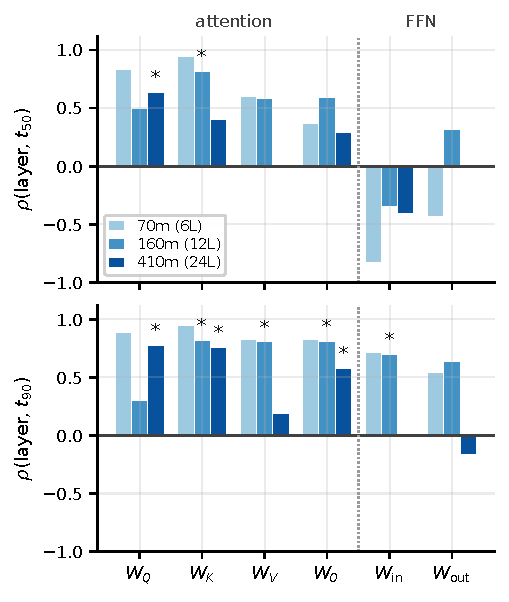
\includegraphics[width=\columnwidth]{figures/fig0_depth_summary.pdf}
% \caption{Spearman correlation between layer index and stabilization step for
% each matrix type (top $\tf$, bottom $\tn$). Positive means deeper layers
% settle later. $^{*}$: $p<0.05$ after Holm correction over the six matrix
% types. Attention is positive under both measures; $\Win$ is negative under
% $\tf$ and positive or flat under $\tn$.}
% \label{fig:scale}
% \end{figure}

% \paragraph{H2: not supported.} On Pythia-70m and 160m attention and the FFN
% settle at the same time under both measures ($r = \HtwoRSmall$,
% $p \HtwoPSmall$ at 70m; $r = \HtwoRBig$, $p \HtwoPBig$ at 160m, with attention
% earlier in \HtwoLowerBig{} of \HtwoPairsBig{} layers). On Pythia-410m the FFN
% is earlier under $\tf$ (attention earlier in only \HtwoLowerHuge{} of
% \HtwoPairsHuge{} layers, $r = \HtwoRHuge$, $p \HtwoPHuge$), but under $\tn$
% the difference is not significant ($r = \HtwoRHugeNinety$,
% $p \HtwoPHugeNinety$), so it is not robust. Attention does not settle before
% the FFN at any size.

% \paragraph{H3: not supported; $\Wo$ settles first.} On Pythia-410m the four
% attention matrices differ strongly (Friedman $\chi^2 = \HthreeChiHuge$,
% $p \HthreePHuge$, Kendall's $W = \HthreeWHuge$), but not in the predicted
% order. The median $\tf$ of $\Wo$ is \HthreeOMedHuge{} steps, against
% \HthreeQMedHuge{}, \HthreeKMedHuge{} and \HthreeVMedHuge{} for $\Wq$, $\Wk$
% and $\Wv$, and $\Wo$ is earlier than each of the other three in the
% Holm-corrected pairwise tests under both measures. The planned contrast
% therefore puts $(\Wq,\Wk)$ \emph{later} than $(\Wv,\Wo)$ at 410m
% ($r = \HthreeCRHuge$ under $\tf$ and $\HthreeCRHugeNinety$ under $\tn$, both
% $p < 0.001$). This comes from $\Wo$ alone: $\Wv$ is not earlier than $\Wq$ and
% $\Wk$, and under $\tf$ it is even later than $\Wk$ ($r = \HthreeKVRHuge$,
% $p_{\text{Holm}} \HthreeKVPHuge$). On 160m the $\Wo$-first pattern holds under
% $\tf$ ($p \HthreeCPBig$) but not under $\tn$ ($p \HthreeCPBigNinety$), and 70m
% shows no significant difference. The result is therefore narrower than a
% QK-versus-OV ordering: the attention output projection reaches its final
% direction first, clearly so at 410m.

% \paragraph{H4: only for the output embedding, at the two smaller sizes.} On
% Pythia-70m and 160m the output embedding is the last of all tracked matrices
% to settle, under both measures ($\tf = \EmbOutTfiftyBig$ steps on 160m). The
% input embedding is not late: on 160m under $\tf$ the input and output
% embeddings rank \HfourRanksBig{} of \HfourPoolBig{} (1 = latest). At 410m the
% answer depends on the measure. Under $\tf$ both embeddings rank early
% (\HfourRanksHuge{} of \HfourPoolHuge{}), and under $\tn$ both rank late
% (\HfourRanksHugeNinety{}, $p \HfourPHugeNinety$). The two embeddings clearly
% do not behave as one group.

% \paragraph{H5: partly supported.} The Spearman correlations between the
% models' $\log_{10}\tf$ depth profiles are $+0.76$ (70m--160m), $+0.57$
% (160m--410m) and $+0.35$ (70m--410m), so agreement falls as the size gap
% grows. The signs of H1--H3 agree across models under $\tf$, but for H2 and H3
% not under $\tn$.

% \paragraph{Weight change slows gradually.} The displacement rate $r_t$ falls
% smoothly during training, by about 50--80$\times$ from its early peak to the
% end, with no sudden drop. Almost every matrix does eventually stay below the
% smallest threshold we tried ($\tau = \TauMin$, i.e.\ 2\% relative change per
% 1000 steps): \TauBelowNSmall{} of \NMatSmall, \TauBelowNBig{} of \NMatBig{}
% and \TauBelowNHuge{} of \NMatHuge{} matrices. But this happens late, between
% steps \TauBelowMinHuge{} and \TauBelowMaxBig{} (median \TauBelowMedHuge{} at
% 410m). A ``stabilization step'' defined by a threshold is therefore a point on
% a gradual slowdown, and where it falls depends on $\tau$.

\FloatBarrier
\begin{table*}[t]
\centering\small
\setlength{\tabcolsep}{5pt}
\begin{tabular}{l rr rr rr}
\toprule
 & \multicolumn{2}{c}{\textbf{Pythia-70m} (6 layers)}
 & \multicolumn{2}{c}{\textbf{Pythia-160m} (12 layers)}
 & \multicolumn{2}{c}{\textbf{Pythia-410m} (24 layers)} \\
\cmidrule(lr){2-3}\cmidrule(lr){4-5}\cmidrule(lr){6-7}
\textbf{Statement tested}
 & halfway & 90\% & halfway & 90\% & halfway & 90\% \\
\midrule
(H1) Deeper layers settle later: all matrices
 & \HoneRhoSmall\HoneSigSmall & \HoneRhoSmallNinety\HoneSigSmallNinety
 & \HoneRhoBig\HoneSigBig & \HoneRhoBigNinety\HoneSigBigNinety
 & \HoneRhoHuge\HoneSigHuge & \HoneRhoHugeNinety\HoneSigHugeNinety \\
(H1) Deeper layers settle later: $\Wq$ only
 & \HoneRhoQSmall\HoneSigQSmall & \HoneRhoQSmallNinety\HoneSigQSmallNinety
 & \HoneRhoQBig\HoneSigQBig & \HoneRhoQBigNinety\HoneSigQBigNinety
 & \HoneRhoQHuge\HoneSigQHuge & \HoneRhoQHugeNinety\HoneSigQHugeNinety \\
(H1) Deeper layers settle later: $\Win$ only
 & \HoneRhoFinSmall\HoneSigFinSmall & \HoneRhoFinSmallNinety\HoneSigFinSmallNinety
 & \HoneRhoFinBig\HoneSigFinBig & \HoneRhoFinBigNinety\HoneSigFinBigNinety
 & \HoneRhoFinHuge\HoneSigFinHuge & \HoneRhoFinHugeNinety\HoneSigFinHugeNinety \\
(H2) The FFN settles before attention
 & \HtwoRSmall\HtwoSigSmall & \HtwoRSmallNinety\HtwoSigSmallNinety
 & \HtwoRBig\HtwoSigBig & \HtwoRBigNinety\HtwoSigBigNinety
 & \HtwoRHuge\HtwoSigHuge & \HtwoRHugeNinety\HtwoSigHugeNinety \\
(H3) $\Wv, \Wo$ settle before $\Wq, \Wk$
 & \HthreeCRSmall\HthreeCSigSmall & \HthreeCRSmallNinety\HthreeCSigSmallNinety
 & \HthreeCRBig\HthreeCSigBig & \HthreeCRBigNinety\HthreeCSigBigNinety
 & \HthreeCRHuge\HthreeCSigHuge & \HthreeCRHugeNinety\HthreeCSigHugeNinety \\
\bottomrule
\end{tabular}
\caption{Phase~1 results. ``Halfway'' and ``90\%'' are the two settling times
($\tf$ and $\tn$). Each value runs from $-1$ to $+1$: positive means the
statement holds, negative means the opposite holds, and 0 means no pattern.
$^{*}$: statistically significant ($p<0.05$; the $\Wq$ and $\Win$ rows are
corrected for testing six matrix types). H2 and H3 are phrased so that a
positive value is the \emph{opposite} of what we predicted.}
\label{tab:p1}
\end{table*}

\paragraph{H1: bottom-up for attention, not for the FFN.} Overall, deeper
layers settle later, but clearly so only at 160m; at 70m the six layers are
too few for a significant result. Figure~\ref{fig:scale} shows why the trend
is weak elsewhere. The attention matrices settle later in deeper layers at
every size and under both measures, while the FFN does not: in upper layers
it gets halfway to its final direction early but does not finish early. Under
the halfway measure this pulls the overall trend down, most visibly at 410m.
The bottom-up ordering is therefore a property of attention.

\begin{figure}[t]
\centering
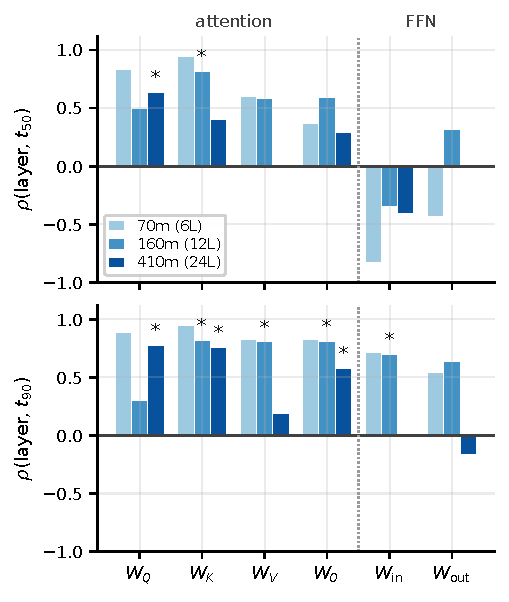
\includegraphics[width=\columnwidth]{figures/fig0_depth_summary.pdf}
\caption{How strongly deeper layers settle later, for each matrix type and
model size (top: halfway, bottom: 90\%). Positive means deeper layers settle
later. $^{*}$: statistically significant after correcting for six matrix
types. Attention is positive under both measures; $\Win$ is negative at
halfway and positive or flat at 90\%.}
\label{fig:scale}
\end{figure}

\paragraph{H2: not supported.} Attention does not settle before the FFN at
any size. At 70m and 160m the two settle at the same time. At 410m the FFN is
earlier by the halfway measure but not significantly by the 90\% measure, so
we do not treat it as a real effect.

\paragraph{H3: not supported; $\Wo$ settles first.} The last row of
Table~\ref{tab:p1} is mostly positive, the opposite of the prediction, but this comes
from $\Wo$ alone. At 410m $\Wo$ reaches halfway after \HthreeOMedHuge{} steps
(median over layers), against \HthreeQMedHuge--\HthreeVMedHuge{} for the other
three, and it is significantly earlier than each of them under both measures.
$\Wv$ is not earlier than $\Wq$ and $\Wk$. At 160m this holds only for the
halfway measure, and at 70m not at all. So the attention output matrix settles
first, but there is no general ``where to look'' before ``what to move''
ordering.

% \paragraph{H4: only for the output embedding, at the two smaller sizes.} At 70m
% and 160m the output embedding is the last of all tracked matrices to settle,
% under both measures, while the input embedding is not late. At 410m the result
% depends on the measure: both embeddings are among the earliest at halfway and
% among the latest at 90\%. The two embeddings do not behave as one group.

% \paragraph{H5: partly supported.} Models of similar size show similar
% patterns, and the similarity drops as the size gap grows. Comparing the
% models' settling times along depth for every matrix type gives a correlation
% of $+0.76$ for 70m--160m, $+0.57$ for 160m--410m and $+0.35$ for 70m--410m.
% The directions in Table~\ref{tab:p1} agree across sizes at halfway, but not
% always at 90\%.

% \paragraph{H4: only for the output embedding, at the two smaller sizes.} We
% rank all tracked matrices of a model by settling time (1 = last to settle).
% At 70m and 160m the output embedding has rank 1 under both measures, while the
% input embedding is not late (input and output ranks \HfourRanksSmall{} of
% \HfourPoolSmall{} at 70m and \HfourRanksBig{} of \HfourPoolBig{} at 160m,
% halfway measure). At 410m the result depends on the measure: ranks
% \HfourRanksHuge{} of \HfourPoolHuge{} at halfway, \HfourRanksHugeNinety{} at
% 90\%. The two embeddings do not behave as one group.

% \paragraph{H5: partly supported.} For each model we take the settling times of
% every matrix type along the depth of the model, and correlate these profiles
% between models (Figure~\ref{fig:overlay} in the appendix shows them). The
% correlation is $+0.76$ for 70m--160m, $+0.57$ for 160m--410m and $+0.35$ for
% 70m--410m, so models of similar size behave similarly and the similarity drops
% as the size gap grows. The directions in Table~\ref{tab:p1} agree across sizes
% at halfway, but not always at 90\%.

\begin{table}[t]
\centering\small
\begin{tabular}{l rr rr}
\toprule
 & \multicolumn{2}{c}{\textbf{Input embedding}} & \multicolumn{2}{c}{\textbf{Output embedding}} \\
\cmidrule(lr){2-3}\cmidrule(lr){4-5}
\textbf{Model} & halfway & 90\% & halfway & 90\% \\
\midrule
Pythia-70m  &  5 & 84 & 100 & 100 \\
Pythia-160m & 12 & 52 & 100 & 100 \\
Pythia-410m & 23 & 83 &   6 &  89 \\
\bottomrule
\end{tabular}
\caption{H4: how late each embedding settles, as the percentage of all other
tracked matrices that settle before it (100 = the last of all, 0 = the first
of all).}
\label{tab:h4}
\end{table}

\paragraph{H4: only for the output embedding, at the two smaller sizes.}
Table~\ref{tab:h4} shows that at 70m and 160m the output embedding is the last
matrix to settle under both measures, while the input embedding is not late.
At 410m the answer depends on the measure: both embeddings are among the
earlier matrices at halfway but among the later ones at 90\%. So the two
embeddings do not behave as one group, and only the output embedding supports
H4.

\paragraph{H5: partly supported.} To compare model sizes, we correlate the
depth patterns of settling times between two models: 1 would mean the same
pattern, 0 no relation. The correlation is $+0.76$ between 70m and 160m, $+0.57$ between
160m and 410m, and $+0.35$ between 70m and 410m. Models of similar size
therefore behave similarly, and the similarity drops as the size difference
grows. In Table~\ref{tab:p1}, the direction of each result is the same for all
three sizes at halfway, but not always at 90\%.

\paragraph{Weight change slows gradually.} No matrix stops changing at a clear
point. The rate of change falls smoothly, by about 50--80$\times$ over
training. Almost every matrix eventually stays below 2\% change per 1000 steps
(\TauBelowNHuge{} of \NMatHuge{} at 410m), but only after step
\TauBelowMinHuge{}. A looser limit gives a much earlier ``stopping'' step, so
any stabilization step depends on the limit chosen.

% ===========================================================================
\section{Phase 2: Intervening}
% ===========================================================================

% \subsection{From measurements to a schedule}

% Phase~1 gives, for every layer, the step at which its attention matrices
% reached $\tf$ in Pythia's \FinalStep{}-step run. We move it to a Phase~2 run of
% $T$ steps by relative progress: $\sigma(\ell) = \tf(\ell, \text{attn}) /
% \FinalStep$, and layer $\ell$ switches at step $\sigma T$. Both the attention
% and the FFN of that layer switch at this point; the FFN's own $\tf$ is not
% used. Phase~2 trains models of the 70m size, so it uses the 70m measurements.
% This puts the switch near step 310 of 4,000 for layers 0--2 and between steps
% 650 and 860 for layers 3--5.

\subsection{Experimental setup}

We train GPT-NeoX models with the \texttt{pythia-70m} configuration (6 layers,
$d = 512$, 8 heads, rotary embeddings \citep{su2024roformer}; \PhaseTwoParams{}M
parameters) from scratch on WikiText-103 \citep{merity2017pointer}, using its
official train/validation split. The test split is not used. We tokenize the
non-empty lines with the Pythia tokenizer, join them with an end-of-text token,
and cut the stream into 512-token blocks. This gives 119.9M training and 252K
validation tokens. Every evaluation uses the same first 196,608 validation
tokens. We report validation perplexity: the exponential of the average
per-token cross-entropy loss, where lower is better.

We use AdamW \citep{loshchilov2019adamw} ($\beta = 0.9, 0.95$; weight decay
0.1; gradient clipping 1.0) with base learning rate $6\times10^{-4}$, for
\PhaseTwoSteps{} steps of \PhaseTwoTokensPerStep{} tokens (\PhaseTwoTokens{}M
tokens, less than one epoch, so no training block is seen twice). The learning
rate $g(t)$ rises linearly over the first 200 steps and then follows a cosine
decay. As a sanity check, the model can memorize \OverfitBatches{} fixed
training batches (loss $\OverfitStart \rightarrow \OverfitFinal$), so the
training code works.

\subsection{From measurements to a schedule}

Each Phase~2 schedule changes the learning rate of a layer at one
\emph{switch step}. We take this step from Phase~1: it is the time at which
that layer's attention matrices got halfway to their final direction ($\tf$)
in Pythia-70m, the same model size we train. Pythia trained for
\FinalStep{} steps and our models for \PhaseTwoSteps{}, so we keep the same
fraction of training. For example, layer~0's attention reached halfway after
about 11,200 of \FinalStep{} steps (7.9\%), so layer~0 switches at step 314 of
\PhaseTwoSteps{}. This gives a switch near step 310 for layers 0--2 and
between steps 650 and 860 for layers 3--5, so deeper layers switch later.
In each layer, the attention and the FFN switch at the same step.

\subsection{Arms}\label{sec:arms}
We compare several versions of training, which we call \emph{arms}. All arms use the setup above and differ only in their
learning rate: each arm multiplies $g(t)$ by a factor $m(t,\ell)$ for the
attention or FFN parameters of layer $\ell$. Embeddings and layer norms always
use $g(t)$.

\begin{itemize}\itemsep0pt \parskip0pt
\item \textbf{baseline}: $m = 1$ everywhere.
\item \textbf{attn-first}: attention uses $m = A$ before its layer's switch
  point and $m = B$ after, with $B = A/3$; the FFN gets the mirror image.
\item \textbf{attn-second}: the mirror of attn-first (FFN emphasised first).
\item \textbf{attn-first-lrm, attn-second-lrm}: the same profiles, with $A$
  and $B$ chosen so that each group's total learning rate
  $\sum_t g(t)\,m(t,\ell)$ equals the baseline's.
\item \textbf{alternating}: the emphasis swaps between attention and FFN every
  200 steps. It uses no Phase~1 input and tests whether separating the two
  groups helps by itself.
\item \textbf{attn-freeze}: attention's learning rate is set to 0 after its
  switch point. This tests freezing directly and is not budget-matched.
\end{itemize}

In attn-first and attn-second, $A$ and $B$ were chosen so that the
\emph{average} multiplier over training steps is 1, as in the baseline. This
does not give each group the same total learning rate, because $g(t)$ is not
flat. The group emphasised early, when $g$ is largest, receives
\BudgetEarlyPct\% more total learning rate than in the baseline, and the
other group \BudgetLatePct\% less. We added the two \texttt{-lrm} arms after
finding this imbalance. They remove it exactly, which separates the effect of
timing from the effect of the budget.

\paragraph{Why emphasis instead of freeze-then-unfreeze.} Originally we planned
to freeze the parts of a block that settle later, train only the parts that
settle first, and unfreeze the rest once those had stabilized. Phase~1 removed
the basis for this: at 70m attention and the FFN settle at the same time, and
no matrix stops changing at a clear point that could trigger the unfreeze.
We therefore changed how strongly each group is trained over time instead of switching groups off, and kept one freezing arm (attn-freeze) to measure the possible compute saving.

% \subsection{Experimental setup}

% We train GPT-NeoX models with the \texttt{pythia-70m} configuration (6 layers,
% $d = 512$, 8 heads, rotary embeddings \citep{su2024roformer}; \PhaseTwoParams{}M
% parameters) from scratch on WikiText-103 \citep{merity2017pointer}, using its
% official train/validation split. The test split is not used. We tokenize the
% non-empty lines with the Pythia tokenizer, join them with an end-of-text token,
% and cut the stream into 512-token blocks. This gives 119.9M training and 252K
% validation tokens. Every evaluation uses the same first 196,608 validation
% tokens. We report validation perplexity: the exponential of the average
% per-token cross-entropy loss, where lower is better.

% We use AdamW \citep{loshchilov2019adamw} ($\beta = 0.9, 0.95$; weight decay
% 0.1; gradient clipping 1.0) with base learning rate $6\times10^{-4}$, for
% \PhaseTwoSteps{} steps of \PhaseTwoTokensPerStep{} tokens (\PhaseTwoTokens{}M
% tokens, less than one epoch, so no training block is seen twice). All
% hyperparameters are the same for every arm.

\subsection{Comparing the arms}
Each arm is trained several times with different random \emph{seeds}. The
seed fixes the random starting weights and the order in which training
batches are drawn, so different seeds give different but equally valid runs.
We use six seeds (0--5) for the baseline and the four directed arms
(attn-first, attn-second and their \texttt{-lrm} versions), and three seeds
(0--2) for alternating and attn-freeze, \PhaseTwoRuns{} runs in total. Six is
the smallest number of seeds for which a result where every seed agrees can
reach $p < 0.05$ (see below); the two side arms got three to save
compute.
For a given seed, every arm starts from the same initialization and sees the same batches in the same order; only the
learning-rate factors differ.
% A weight-displacement probe recorded in every
% run shows that each arm changed the intended parameters
% (Figure~\ref{fig:disp}).

We compare each arm to the baseline paired by seed. To test whether an arm differs from the baseline, we take the difference
(arm minus baseline) for each seed. If the arm had no effect, each difference
would be equally likely to be positive or negative, so we flip the signs of
the differences in all possible ways and count how often the average is at
least as far from zero as the real one; that fraction is the $p$-value. When
all seeds agree in direction, this gives the smallest possible $p$: $2/64 =
0.031$ with six seeds, and $2/8 = 0.25$ with three, which can never be
significant. A $p$ of 0.031 therefore means ``every seed agreed''. The main metrics are the number of steps to reach
validation perplexity \TargetPpl{} and the final validation perplexity. The
target \TargetPpl{} is set by rule, as the lowest round number reached by
every run of baseline, attn-first and attn-second. $p$-values are not corrected
for the several arms and metrics, so we rely mainly on whether all seeds agree
in sign.

\subsection{Results}
\label{sec:results-p2}

% Phase 2 results. Every number resolves through a macro in numbers.tex,
% written by make_report_numbers.py from the run records.

\begin{table*}[t]
\centering\small
\begin{tabular}{lrrrrrr}
\toprule
\textbf{arm} & \textbf{seeds} & \textbf{final val ppl} & \textbf{steps to 45} & \textbf{sec to 45} & \textbf{train s} & \textbf{peak GiB} \\
\midrule
baseline & 6 & 40.54 {\scriptsize$\pm$ 0.33} & 2,915 {\scriptsize$\pm$ 48} & 381 & 523 & 7.40 \\
attn-first & 6 & 41.63 {\scriptsize$\pm$ 0.81} & 3,096 {\scriptsize$\pm$ 165} & 405 & 523 & 7.40 \\
attn-second & 6 & 40.16 {\scriptsize$\pm$ 0.15} & 2,774 {\scriptsize$\pm$ 23} & 363 & 524 & 7.40 \\
attn-first-lrm & 6 & 41.07 {\scriptsize$\pm$ 0.60} & 2,993 {\scriptsize$\pm$ 103} & 389 & 520 & 7.40 \\
attn-second-lrm & 6 & 40.21 {\scriptsize$\pm$ 0.17} & 2,788 {\scriptsize$\pm$ 22} & 365 & 523 & 7.40 \\
alternating & 3 & 40.65 {\scriptsize$\pm$ 0.56} & 2,914 {\scriptsize$\pm$ 85} & 385 & 530 & 7.40 \\
attn-freeze & 3 & 53.91 {\scriptsize$\pm$ 0.56} & --- & --- & 512 & 7.40 \\
\bottomrule
\end{tabular}
\caption{Phase~2 results, mean $\pm$ SD over seeds. ``steps to 45'' and ``sec to 45'' are the training step and training seconds at which validation perplexity first reaches 45 (interpolated; --- if never reached). ``train s'' is total training time and ``peak GiB'' the peak GPU memory. At a given seed every arm shares the baseline's initialization and data order.}
\label{tab:p2}
\end{table*}


\begin{figure}[t]
\centering
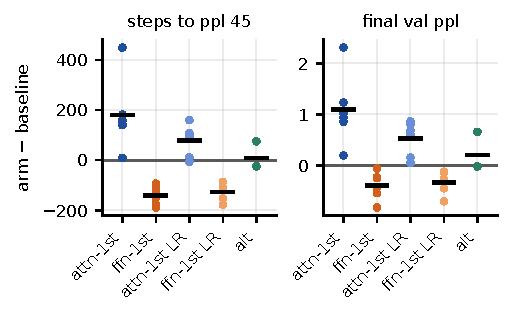
\includegraphics[width=\columnwidth]{figures/figp_paired.pdf}
\caption{Per-seed differences from the baseline (each point is one seed; the
bar is the mean). 
Left shows difference in step count to reach perplexity 45. 
Right shows difference in final perplexity value.
Below zero means the arm beat the baseline for that seed.
``LR'' marks the learning-rate-matched arms. attn-freeze (+13 perplexity) is
left out for scale.}
\label{fig:paired}
\end{figure}

Table~\ref{tab:p2} lists every arm, and Figure~\ref{fig:paired} shows the
per-seed differences from the baseline.

% \paragraph{FFN first helps.} attn-second beats the baseline in all
% \ASStepsNseeds{} seeds: \ASStepsDiffAbsInt{} fewer steps to perplexity
% \TargetPpl{} ($-\ASStepsRelAbs$\%, $p \ASStepsP$) and $-\ASPplRelAbs$\% final
% perplexity ($p \ASPplP$). This arm also gives the FFN \BudgetEarlyPct\% more
% total learning rate than the baseline, so the gain could come from the larger
% budget alone. attn-second-lrm removes that difference and keeps most of the
% gain: $-\ASLStepsRelAbs$\% steps and $-\ASLPplRelAbs$\% final perplexity, again
% better than the baseline in every seed ($p \ASLStepsP$ for both). The
% advantage of emphasising the FFN early is therefore not a budget effect.

% \paragraph{Attention first hurts.} attn-first is worse than the baseline in
% every seed ($+\AFStepsRelAbs$\% steps, $+\AFPplRelAbs$\% final perplexity,
% $p \AFStepsP$ for both). With the budget matched, attn-first-lrm is still
% worse, by about half as much: $+\AFLStepsRelAbs$\% steps (worse in
% \AFLStepsWorse{} of \AFLStepsNseeds{} seeds, $p \AFLStepsP$) and
% $+\AFLPplRelAbs$\% final perplexity (\AFLPplWorse{} of \AFLPplNseeds{},
% $p \AFLPplP$). So about half of the original penalty came from the budget.
% Compared directly, the two matched arms separate in \AFLvASLStepsWorse{} of
% \AFLvASLStepsNseeds{} seeds on both metrics ($p \AFLvASLStepsP$).

% These $p$-values are the smallest possible with six seeds, so they mean
% ``every seed agreed'' rather than a precise probability. The effects are
% small: a few percent in steps, about 1\% in final perplexity.

\paragraph{Training the FFN first helps.} Emphasising the FFN before the
switch step makes training faster in every seed: attn-second needs
\ASStepsRelAbs\% fewer steps to reach perplexity \TargetPpl{} and ends with
slightly lower perplexity. This arm also gives the FFN more total learning
rate than the baseline (Section~\ref{sec:arms}), so the gain could have come
from the extra learning rate alone. To check this, attn-second-lrm uses
the same timing with the total learning rate matched to the baseline. It
keeps almost all of the gain (\ASLStepsRelAbs\% fewer steps), again in every
seed. What helps is therefore \emph{when} the FFN is emphasised, not how much
learning rate it gets.

\paragraph{Training attention first hurts.} The mirror image, attn-first, is
slower than the baseline in every seed. About half of this penalty came from
the learning-rate imbalance: with the total matched, attn-first-lrm is still
worse, but by roughly half as much, and no longer in every seed. Compared
directly, the two matched arms still differ in every seed, so the order in
which the two groups are emphasised matters.

\paragraph{How large are these effects?} Small. The best arm saves about
\ASLStepsRelAbs\% of the training steps and improves the final perplexity by
under 1\%. Every seed agrees on the direction, so the effects are consistent,
but they are about how fast the model trains, not how good it becomes.

\paragraph{Alternating has no effect.} alternating is indistinguishable from
the baseline ($\AltPplDiff$ perplexity, $p \AltPplP$; $\AltStepsDiffInt$ steps,
$p \AltStepsP$; \AltSeeds{} seeds) and its curve lies on the baseline's
(Figure~\ref{fig:curves}). Changing the emphasis without the Phase~1 timing
does not help.

\begin{figure}[t]
\centering
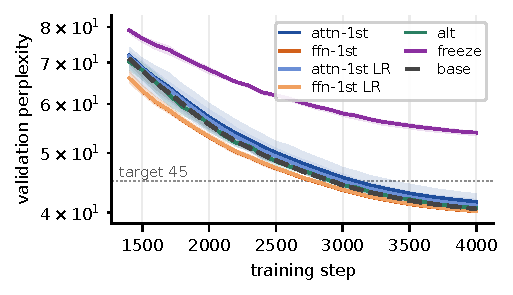
\includegraphics[width=\columnwidth]{figures/figp_curves.pdf}
\caption{Validation perplexity over the last two thirds of training (line:
mean over seeds; band: min--max). The baseline is dashed; alternating lies on
it. Both FFN-first arms (orange) stay below it.}
\label{fig:curves}
\end{figure}

\paragraph{Freezing hurts and saves little.} attn-freeze sets attention's
learning rate to zero after each layer's switch point, which falls 8--21\% of
the way into training. Attention's total weight displacement drops to
\FrzDispAttn{}, against \BaseDispAttn{} in the baseline, so attention really
stops learning. Final perplexity is \FrzPpl{} (\FrzPplRelAbs\% worse), and the
target of \TargetPpl{} is never reached. Training time drops by
\FrzWallRelAbs\% (\FrzWallDiffAbs{}\,s of \BaseWall{}\,s, 3 seeds).

% \paragraph{Manipulation check.} The weight displacement moves as designed
% (Figure~\ref{fig:disp}): attn-first moves attention more than the baseline
% (\AFDispAttn{} vs \BaseDispAttn) and the FFN less (\AFDispFfn{} vs
% \BaseDispFfn); attn-second does the reverse (\ASDispAttn{}, \ASDispFfn).


% ===========================================================================
\section{Discussion}
\label{sec:discussion}
% ===========================================================================

% \paragraph{Phase 1 does not support a within-block schedule.} The depth trend
% of attention is clear at all three sizes, but the orderings inside a block,
% which a matrix-level schedule would use, were not found. Attention and the FFN
% settle at the same time at 70m and 160m, and at 410m the FFN is earlier under
% only one of the two measures. There is no measured ``attention before FFN''
% timing to exploit. The only robust within-block ordering is that $\Wo$
% settles first. The query/key pair, which the circuits view
% \citep{elhage2021framework} suggests should settle first, does not settle
% before $\Wv$.

% \paragraph{The direction of the schedule still mattered.} The two mirrored
% schedules differ only in which group is emphasised early, and they separate in
% all six seeds, in favour of FFN-first. The learning-rate-matched arms rule out
% the simplest explanation, that the winning arm just gave the FFN more learning
% rate, and the alternating control rules out the idea that any separation of
% the groups helps. What the result does not show is \emph{why} FFN-first wins.
% The effect is small (about 4\% of steps) and is about training speed rather
% than final capability. Our design also cannot separate a stabilization-timing
% explanation from a simpler one: the FFN may just benefit more from a high
% learning rate early in training. The switch points came from the 70m
% measurements, where attention and the FFN settle at the same time, so Phase~1
% does not predict this direction. Arms with deliberately wrong switch points,
% or a Phase~2 at 410m, would be needed to tell the two apart.

\paragraph{What Phase 1 shows.} We found two clear orderings. Across layers,
attention settles bottom-up at every model size. Inside a block, the attention
output matrix $\Wo$ settles before the other attention matrices, clearly so at
410m. Between attention and the FFN the picture depends on scale: at 70m and
160m they settle together, and at 410m the FFN tends to settle first, though
only under the halfway measure. This is not the ``routing before memory''
order we expected, and the query/key pair, which our H3 predicted would settle
first based on the QK/OV split of \citet{elhage2021framework}, does not.

\paragraph{The order of emphasis matters for training speed.} In Phase~2,
emphasising the FFN before attention trained faster than the baseline in every
seed, and emphasising attention first was slower. The learning-rate-matched
arms show that this comes from the timing of the emphasis, not from giving the
FFN more learning rate, and the alternating control shows that switching
emphasis by itself does not help. A simple per-layer change of learning rates,
with no extra compute, consistently reached the target about 4\% sooner. It
is also the same order that Phase~1 hints at for the largest model.

\paragraph{What remains open.} The gain is small and is about training speed
rather than final quality. We also cannot yet say why it works. The switch
points came from 70m, where attention and the FFN settle together, so the
gain may simply mean that the FFN benefits more from a high learning rate
early in training. Arms with deliberately wrong switch points, or a Phase~2
at 410m, would tell these explanations apart.

\paragraph{Why freezing saved so little.} Reflecting upon the underwhelming results, we believe that even though freezing removes a matrix's weight gradient and optimizer
update, it does not remove the backward pass through that matrix, which
earlier layers still need, or the activations stored for it. The possible
saving was also small from the start: attention is \ParamPctAttn\% of the
parameters, its optimizer state is allocated before the freeze, and peak
memory is dominated by the output logits over a 50K vocabulary. So the result
shows that freezing single matrices buys little in this setting, not that
freezing never helps. 

% ===========================================================================
\section{Limitations}
% ===========================================================================

\begin{itemize}\itemsep0pt \parskip0pt
% \item \textbf{Weights, not behaviour.} We measure when a matrix's weights stop
%   changing direction, not when its effect on the model's output stops
%   changing. Two matrices can point in slightly different directions and still
%   compute almost the same thing, so ``settled weights'' and ``settled
%   behaviour'' are not the same. Checking the second would require comparing
%   the model's internal activations across checkpoints, which we did not do.
  
\item \textbf{The final checkpoint is not a finished model.} Pythia's training
  ends at step \FinalStep{}, so we use that checkpoint as the ``final''
  direction. The matrices are still changing slightly there (about 1\% per
  1000 steps), so the true end state may differ.
  
\item \textbf{Limited model sizes.} We study three Pythia models, trained with
  one recipe, and train our own models only at the 70m size. The 36 training
  runs took about six GPU-hours on a single consumer GPU; repeating them at
  410m would take many times longer, which did not fit the time and hardware
  available to us. Whether the schedules help at larger sizes, and whether
  our findings hold for other model families, remains untested.
  
% \item \textbf{Transfer between phases.} Mapping Pythia's \FinalStep{}-step
%   timings onto a \PhaseTwoSteps{}-step run by relative progress is an
%   assumption, not a measurement.

\item \textbf{Small numbers of seeds and layers.} Six seeds per main arm (three
  for the side arms) and only six layers in the smallest model limit how
  small an effect we can detect, and several Phase~1 results hold under only
  one of our two measures.
  
\item \textbf{Learning rate and weight decay change together.} In PyTorch's
  AdamW implementation, which we use, weight decay is multiplied by the
  learning rate, so a per-group multiplier also changes that group's weight
  decay. Part of an
  effect could come from regularization.

\item \textbf{Simplifying assumptions.} Several steps rely on simple rules
  rather than measurements. We move switch steps from Pythia's
  \FinalStep{}-step run to our \PhaseTwoSteps{}-step runs by keeping the same
  fraction of training, which assumes both runs progress at the same relative
  pace. Settling times between checkpoints are estimated by drawing a straight
  line between the two nearest checkpoints. Each matrix is treated as a single
  direction, and each layer is summarized by the median of its matrices. The
  emphasis ratio of 3 and the use of attention's switch step for both groups
  were fixed choices that we did not vary.
  We also combine all attention heads of a layer into one $\Wq$, $\Wk$ and
$\Wv$, so differences between individual heads are not visible.
  
\end{itemize}

% ===========================================================================
\section{AI Disclosure and Reflection}
% ===========================================================================

The research question, the two-phase design and the interpretation of the
results are ours, and we take responsibility for everything in this paper.
We used Claude (Anthropic; Opus~5 and Opus~5.5, through the Claude Code tool)
to write code quickly, to learn background we did not know well such as
Transformer internals and training procedures, to rapidly develop code, tests and logging, and to help draft and edit the paper text. We also used it to find the paper references for specific claims or techniques we used (and we've made sure to verify each quoted paper). We also wanted to adhere to professional standards in our statistical methodology, having well defined hypotheses and clear p values so we can make substantiated claims - the AI guided us on which correct statistical tools to use and how.
These made the implementation much faster, but its output still had to be checked. We verified all the code written and didn't blindly rely on the AI at any point.

% a review
% of the code found that our first emphasis schedules did not give each group
% the same total learning rate, which is why we added the learning-rate-matched
% runs.

% ===========================================================================
\section{Conclusion}
% ===========================================================================

We measured when each weight matrix of a Transformer block settles during
pretraining, and used these measurements to build training schedules. We found
that attention matrices settle bottom-up at all three model sizes, and that
inside the attention block the output matrix $\Wo$ settles first. Attention
and the FFN settle together in the smaller models, while in the largest the
FFN tends to settle first. Weight change slows gradually rather than stopping
at a clear point.

In training, the order of emphasis mattered. Emphasising the FFN early reached
the target perplexity \ASLStepsRelAbs\% faster than the baseline in every
seed, with no extra compute and even with each group's total learning rate
matched, while emphasising attention early was slower. The effect is small,
and why it works is still open: the schedule came from the 70m model, where
attention and the FFN settle together. Freezing attention, in contrast, saved
only \FrzWallRelAbs\% of training time and no memory, at a large cost in
perplexity.

% acl.sty already issues \bibliographystyle{acl_natbib}; repeating it here made
% bibtex abort with "Illegal, another \bibstyle command".
\bibliography{references}

% REMOVING APPENDIX:

% The appendix is single-column so that the wide figures sit next to their
% text instead of being pushed to the following page.
% \clearpage
% \onecolumn
% \appendix

% \section{Reproduction}
% \label{app:repro}

% Every figure and number regenerates from the repository:
% {\small\begin{verbatim}
% python extract_kinematics.py --model <m>
% python compute_stabilization.py --model <m>
% python plot_kinematics.py --all
% python data_prep.py
% sh run_matrix.sh 4000
% python plot_phase2.py
% python make_report_numbers.py
% \end{verbatim}}
% Each Phase~2 run directory stores its full configuration, the schedule
% with the Phase~1 values it came from, the environment, per-step logs,
% evaluation results and the weight-displacement probe. \texttt{demo.sh} runs
% the whole pipeline at toy scale in about three minutes.

% \section{Additional figures}

% The figures below give more detail for Phase~1 (mostly for Pythia-160m;
% the same figures for the other two sizes are in \texttt{figs/}) and the
% Phase~2 training curves and manipulation check.

% \begin{figure}[ht]
% \centering
% \includegraphics[width=0.8\textwidth]{figures/fig5_scale_overlay.pdf}
% \caption{Stabilization step against relative depth for all three models and
% both measures (median over each group's matrices in a layer).
% Figure~\ref{fig:scale} summarises this by matrix type.}
% \label{fig:overlay}
% \end{figure}

% \begin{figure}[ht]
% \centering
% \includegraphics[width=0.8\textwidth]{figures/fig6_matrix_types_pythia160m.pdf}
% \caption{Pythia-160m. Left: $\tf$ by matrix type (grey lines are single
% layers). Right: per-layer log-ratios; above zero means the first-named group
% settles earlier. Attention vs FFN is centred on zero; $(\Wq,\Wk)$ vs
% $(\Wv,\Wo)$ is below zero because of $\Wo$.}
% \label{fig:types}
% \end{figure}

% \begin{figure}[ht]
% \centering
% \includegraphics[width=0.8\textwidth]{figures/fig2_progress_pythia160m.pdf}
% \caption{Directional progress $p_t$ in each layer of Pythia-160m, with
% $\tf$ (circles) and $\tn$ (triangles).}
% \label{fig:progress}
% \end{figure}

% \begin{figure}[ht]
% \centering
% \includegraphics[width=0.8\textwidth]{figures/fig3_wavefront_pythia160m.pdf}
% \caption{Displacement rate per 1000 steps in Pythia-160m, one panel per
% matrix type, layer on the vertical axis; markers give $\tf$ and $\tn$. The
% attention markers move right with depth; the FFN $\tf$ markers are nearly
% vertical.}
% \label{fig:wavefront}
% \end{figure}

% \begin{figure}[ht]
% \centering
% \includegraphics[width=0.8\textwidth]{figures/fig4_depth_pythia160m.pdf}
% \caption{Median stabilization step per layer in Pythia-160m; the band is
% the interquartile range over the layer's matrices and dashed lines mark the
% embeddings. The rise with depth is clear under both measures.}
% \label{fig:depth}
% \end{figure}

% % \begin{figure}[ht]
% % \centering
% % \includegraphics[width=0.5\textwidth]{figures/fig10_phase2_displacement.pdf}
% % \caption{Manipulation check: total relative weight displacement of the
% % attention and FFN parameters in each arm. attn-freeze moves attention about
% % half as much as the baseline.}
% % \label{fig:disp}
% % \end{figure}

\end{document}
